\documentclass[11pt,a4paper,openany]{book}
\usepackage[utf8]{inputenc}
\usepackage[T1]{fontenc}
\usepackage[spanish,es-noshorthands,es-tabla]{babel}
\usepackage{lmodern}
\usepackage[margin=2.4cm]{geometry}
\usepackage{amsmath,amssymb}
\usepackage{graphicx}
\usepackage{booktabs}
\usepackage{tabularx}
\usepackage{xcolor}
\usepackage{enumitem}
\usepackage[most]{tcolorbox}
\usepackage{listings}
\usepackage[hidelinks]{hyperref}
\graphicspath{{../figuras/}}
\setlist{itemsep=2pt,topsep=4pt}
\decimalpoint

\definecolor{azul}{HTML}{1f4e79}
\definecolor{rojo}{HTML}{c0504d}
\definecolor{verde}{HTML}{4f9a5b}
\definecolor{fondo}{HTML}{f4f6f9}

\newtcolorbox{clave}[1][Idea clave]{colback=azul!5,colframe=azul,fonttitle=\bfseries,title=#1,breakable}
\newtcolorbox{aviso}[1][Cuidado]{colback=rojo!5,colframe=rojo,fonttitle=\bfseries,title=#1,breakable}
\newtcolorbox{practica}[1][En la práctica]{colback=verde!5,colframe=verde,fonttitle=\bfseries,title=#1,breakable}
\newtcolorbox{ejercicios}{colback=fondo,colframe=black!40,fonttitle=\bfseries,title=Ejercicios,breakable}

\lstset{basicstyle=\ttfamily\small,backgroundcolor=\color{fondo},frame=single,rulecolor=\color{black!20},
  breaklines=true,columns=fullflexible,keepspaces=true,
  literate={á}{{\'a}}1 {é}{{\'e}}1 {í}{{\'i}}1 {ó}{{\'o}}1 {ú}{{\'u}}1 {ñ}{{\~n}}1 {·}{{$\cdot$}}1 {Á}{{\'A}}1}
\newcommand{\py}[1]{\texttt{#1}}
\newcommand{\E}{\mathbb{E}}

\title{\Huge\bfseries Curso de Trader Profesional\\[6pt]
\Large Riesgo, ejecución y estrategia en renta variable, divisas, materias primas,\\ renta fija, opciones y cripto\\[14pt]
\normalsize con la librería Python \texttt{trader} y scripts de uso diario}
\author{IGR Metrics}
\date{Edición 1.1 · noviembre de 2026}

\begin{document}
\sloppy\emergencystretch=3em
\frontmatter
\maketitle
\begin{tcolorbox}[colback=white,colframe=black!50,title=Aviso]
Este curso es material educativo. No es asesoramiento financiero ni una recomendación de inversión.
Operar con apalancamiento puede hacer perder más que el capital depositado. Los ejemplos usan datos
sintéticos; ninguna cifra es una predicción ni un resultado real.
\end{tcolorbox}
\tableofcontents
\mainmatter
\chapter{Introducción: qué hace un trader profesional}\label{cap:intro}

Un \emph{trader} profesional no es alguien que adivina hacia dónde va el precio. Es alguien que
\textbf{toma riesgo de forma deliberada, medida y repetible} a cambio de una expectativa positiva, y que
sobrevive lo suficiente como para que esa expectativa se materialice. La diferencia con el aficionado
casi nunca está en la idea de entrada; está en el tamaño, en la disciplina para cortar pérdidas, en los
costes y en el registro honesto de lo que funciona.

\section{Los tipos de trader}
\begin{description}
\item[Sell-side (bancos, creadores de mercado).] Dan liquidez a clientes y ganan el diferencial
  compra-venta (\emph{bid-ask}). Su problema principal es gestionar el inventario y cubrir el riesgo
  que acumulan; sus límites se fijan en DV01, delta, vega y VaR.
\item[Buy-side (fondos, gestoras, hedge funds).] Toman posiciones direccionales o de valor relativo para
  generar rentabilidad. Se miden por Sharpe, drawdown y correlación con el mercado.
\item[Prop trading y traders independientes.] Arriesgan capital propio (o de una firma que les fondea)
  con reglas de pérdida diaria y \emph{drawdown} máximo muy estrictas.
\item[Sistemáticos (\emph{quants}).] Codifican las reglas y dejan que un ordenador las ejecute; su
  ventaja está en la investigación y en la ejecución, y su riesgo en el sobreajuste.
\end{description}

\section{La ecuación del trader}
Si cada operación arriesga una unidad $1R$ (la pérdida si salta el stop), la \emph{esperanza} por
operación es
\begin{equation}\label{eq:esperanza}
  E = p\cdot \bar G - (1-p)\cdot \bar P \qquad (\text{en } R),
\end{equation}
con $p$ la tasa de acierto, $\bar G$ la ganancia media y $\bar P$ la pérdida media (en $R$). El
resultado anual es aproximadamente $E \times N \times (\text{riesgo por operación})$, con $N$ el número
de operaciones. Todo el curso trata de mejorar uno de esos tres factores sin destruir los otros:
\begin{itemize}
\item subir $E$: mejores ideas, mejor ejecución, menos costes (capítulos~\ref{cap:micro}, \ref{cap:tecnico}, \ref{cap:equity}--\ref{cap:cripto});
\item que $E$ sea \emph{real} y no un artefacto del backtest (capítulo~\ref{cap:backtest});
\item elegir el riesgo por operación que maximiza el crecimiento sin arruinarse (capítulo~\ref{cap:riesgo});
\item ejecutar el plan sin que las emociones lo rompan (capítulo~\ref{cap:psico}).
\end{itemize}

\begin{clave}
Una tasa de acierto del 35~\% puede ser excelente si las ganancias medias son 3 veces las pérdidas
($E = 0{,}35\cdot3 - 0{,}65 = 0{,}40R$). Un 80~\% de acierto puede ser ruinoso si cada pérdida es 5
veces la ganancia media. \textbf{El acierto, solo, no significa nada.}
\end{clave}

\section{Cómo usar este curso}
Cada capítulo combina teoría, fórmulas y un enlace a funciones de la librería \py{trader}
(carpeta \py{curso\_trader/}). Las fórmulas que ves aquí son las que están implementadas y
verificadas por los tests. Para instalar y comprobar:
\begin{lstlisting}
cd curso_trader
pip install -r requirements.txt
pytest tests                      # ~15 s, sin red
python scripts/generar_figuras.py # regenera las figuras de este PDF
\end{lstlisting}
Los scripts de \py{scripts/} están pensados para el día a día (capítulo~\ref{cap:rutina}):
tamaño de posición, hoja premercado, informe de riesgo, backtest, diario de operaciones y
calculadoras por clase de activo. Todos funcionan en modo demostración con datos sintéticos y aceptan
tus propios CSV.

\paragraph{Estructura.} La parte~I cubre lo común a todos los mercados (microestructura, estadística,
análisis técnico, riesgo, backtesting y psicología). La parte~II recorre las clases de activo:
\textbf{renta variable (equity)}, \textbf{divisas (FX)}, \textbf{materias primas (commodities)}, y además
\textbf{renta fija}, \textbf{opciones y volatilidad} y \textbf{cripto}, porque un trader de cualquier
mesa necesita entender tipos de interés y opciones. La parte~III convierte todo en una rutina diaria y
un plan de estudio de 12 semanas.

\part{Fundamentos comunes a todos los mercados}
\chapter{Microestructura y ejecución}\label{cap:micro}

\section{El libro de órdenes}
Un mercado electrónico es un \textbf{libro de órdenes limitadas}: a cada precio hay una cola de
órdenes de compra (\emph{bid}) y de venta (\emph{ask} u \emph{offer}). El mejor bid y el mejor ask
forman la horquilla (\emph{spread}); el precio medio es $m = (b+a)/2$. Quien envía una orden a mercado
\emph{cruza} el spread y paga liquidez; quien deja una orden limitada la \emph{provee} y espera.

\begin{table}[h]\centering\small
\begin{tabularx}{\textwidth}{lX}
\toprule
Orden & Uso \\ \midrule
Mercado & Ejecución inmediata al precio disponible. Riesgo: deslizamiento (\emph{slippage}) en libros finos o en noticias. \\
Limitada & Precio máximo (compra) o mínimo (venta). Riesgo: no ejecutarse justo cuando el precio se va. \\
Stop (stop-market) & Se convierte en orden a mercado al tocar el nivel. Garantiza salida, no precio (\emph{gaps}). \\
Stop-limit & Se convierte en limitada al tocar el nivel. Garantiza precio, no salida: peligrosa para stops de protección. \\
OCO / bracket & Objetivo y stop enlazados: si se ejecuta uno se cancela el otro. \\
Iceberg & Muestra solo una parte del tamaño. \\
Validez & DAY, GTC (hasta cancelar), IOC (lo que se pueda ya), FOK (todo o nada), MOC/LOC (al cierre). \\
\bottomrule
\end{tabularx}
\caption{Tipos de orden habituales.}
\end{table}

\section{Costes de transacción}
El coste total de una operación tiene tres partes:
\begin{equation}
\text{coste} = \underbrace{\tfrac12\,\text{spread}}_{\text{explícito}} + \text{comisiones} + \underbrace{\text{impacto}}_{\text{implícito}} .
\end{equation}
El impacto de mercado de una orden grande crece aproximadamente con la \textbf{raíz cuadrada} del
tamaño relativo al volumen diario (ley empírica de la raíz cuadrada):
\begin{equation}\label{eq:impacto}
\frac{\Delta P}{P} \approx Y\,\sigma_{\text{diaria}}\sqrt{\frac{Q}{V}},\qquad Y\approx 0{,}5\text{--}1,
\end{equation}
donde $Q$ es la cantidad y $V$ el volumen diario. Ejemplo: con $\sigma_{\text{diaria}}=2~\%$ y una orden
del 1~\% del volumen diario, el impacto ronda $0{,}1$--$0{,}2~\%$: \emph{más que el spread} de una acción
líquida. Por eso las órdenes grandes se trocean con algoritmos:
\begin{itemize}
\item \textbf{TWAP}: reparte la orden uniformemente en el tiempo.
\item \textbf{VWAP}: reparte según el perfil de volumen intradía (más al principio y al final de la sesión).
\item \textbf{POV}: participa en un porcentaje fijo del volumen que va apareciendo.
\item \textbf{Implementation shortfall}: minimiza la diferencia con el precio de decisión, equilibrando impacto y riesgo de esperar.
\end{itemize}

\begin{practica}
Mide tu ejecución: anota el \emph{precio de decisión} (cuando decides operar) y el precio medio de
ejecución. La diferencia, en puntos básicos, es tu \emph{slippage}. En el backtest
(\py{trader.backtest.backtest}, argumento \py{cost\_bps}) usa un coste igual o mayor al que realmente
pagas; si la estrategia deja de funcionar con el doble de coste, no tiene margen de seguridad.
\end{practica}

\section{Sesiones y liquidez}
\begin{itemize}
\item \textbf{Acciones}: subasta de apertura, sesión continua, subasta de cierre (el cierre concentra
  el 10--20~\% del volumen en EE.~UU. y es el precio de referencia de índices y fondos). Pre y
  post-mercado con poca liquidez.
\item \textbf{FX}: mercado OTC 24 horas de domingo noche a viernes noche; liquidez máxima en el solape
  Londres--Nueva York (aprox. 12--16~h UTC). Fixing WM/Reuters de las 16:00 de Londres.
  \py{trader.fx.open\_sessions(hora\_utc)} dice qué sesiones están abiertas.
\item \textbf{Futuros}: casi 24 horas en Globex/ICE, pero el volumen se concentra en el horario del
  mercado físico (\emph{pit hours}). El precio de liquidación diario (\emph{settlement}) fija el margen.
\item \textbf{Cripto}: 24/7, con liquidez fragmentada entre plataformas.
\end{itemize}

\section{Apalancamiento y margen}
En futuros, CFD, FX al contado con broker y perpetuos de cripto no pagas el nocional, sino un
\textbf{margen inicial} (típicamente 3--15~\% del nocional). Si las pérdidas reducen la cuenta por debajo
del \textbf{margen de mantenimiento}, el broker pide más fondos (\emph{margin call}) o liquida. El
apalancamiento efectivo de la cuenta es
\[
\text{apalancamiento} = \frac{\sum_i |\text{nocional}_i|}{\text{capital}} ,
\]
y es lo que hay que vigilar, no el margen exigido: un margen del 5~\% permite 20x, lo que no significa
que debas usarlo. \py{scripts/informe\_riesgo.py} lo calcula para tu cartera.

\begin{ejercicios}
\begin{enumerate}
\item Una acción cotiza a 49,98 / 50,02. Compras 2000 acciones a mercado y vendes a mercado al cabo de
  un rato sin que el precio medio se mueva. ¿Cuánto has perdido por el spread? ¿Y en pb del nocional?
\item Con la ecuación~\eqref{eq:impacto} ($Y=0{,}7$, $\sigma=1{,}8~\%$) estima el impacto de comprar el
  5~\% del volumen diario. ¿Cuántos días tendrías que repartir la orden para que el impacto diario sea
  menor que 10 pb?
\item ¿Por qué un stop-limit puede no protegerte en un gap de apertura?
\end{enumerate}
\end{ejercicios}

\chapter{Rentabilidad, volatilidad y estadística}\label{cap:estadistica}

\section{Rentabilidades simples y logarítmicas}
La rentabilidad simple es $r_t = P_t/P_{t-1}-1$ y la logarítmica $\ell_t = \ln(P_t/P_{t-1}) = \ln(1+r_t)$.
Las logarítmicas \emph{suman en el tiempo} ($\ell_{0\to T} = \sum \ell_t$); las simples \emph{suman entre
activos} (la rentabilidad de una cartera es $\sum_i w_i r_i$). Usa la que convenga a cada cálculo y no
las mezcles.

Para precios que incluyen dividendos o cambios de contrato hay que usar series \textbf{ajustadas}
(capítulo~\ref{cap:commodities} para el roll de futuros); si no, aparecen saltos falsos.

\section{Volatilidad}
La volatilidad anualizada es la desviación típica de las rentabilidades escalada por la raíz del
número de periodos por año:
\begin{equation}
\sigma_{\text{anual}} = \sigma_{\text{diaria}}\sqrt{252},\qquad \sigma_{\text{diaria}}\approx \frac{\sigma_{\text{anual}}}{16}.
\end{equation}
La regla del 16 es útil: un activo con 32~\% de volatilidad anual se mueve en torno a un 2~\% diario
(una desviación típica). \py{trader.indicators.realized\_vol} calcula la volatilidad realizada en
ventana móvil; \py{trader.indicators.atr} la mide en unidades de precio (rango verdadero medio), que es
lo que se usa para colocar stops.

La volatilidad \textbf{no es constante}: se agrupa (periodos tranquilos y turbulentos), sube cuando los
precios caen en acciones (efecto apalancamiento) y revierte a la media. Por eso los traders
dimensionan con volatilidad reciente (EWMA, GARCH o ATR) y no con la de los últimos diez años.

\section{Colas gruesas}
Las rentabilidades reales tienen \textbf{colas mucho más gruesas} que la normal: movimientos de 5
desviaciones típicas, que bajo normalidad ocurrirían una vez cada varios miles de años, ocurren varias
veces por década. La figura~\ref{fig:colas} lo muestra con rentabilidades $t$ de Student ($\nu=4$).

\begin{figure}[h]\centering
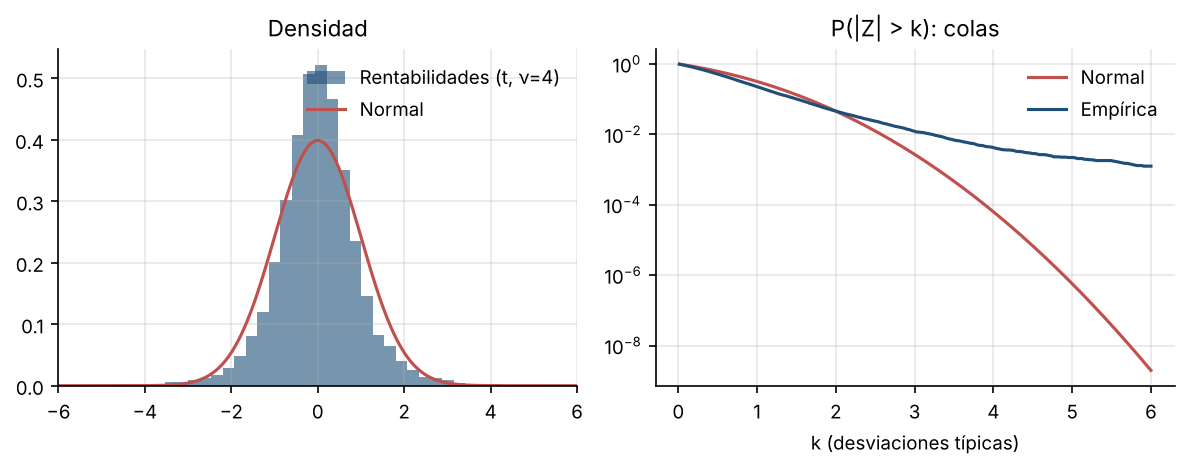
\includegraphics[width=\textwidth]{f02_colas}
\caption{Rentabilidades con colas gruesas frente a la normal. A la derecha, en escala logarítmica, la
probabilidad de superar $k$ desviaciones típicas: la diferencia es de órdenes de magnitud a partir de $k=4$.}
\label{fig:colas}
\end{figure}

\begin{aviso}
Cualquier medida de riesgo que asuma normalidad (VaR paramétrico, Sharpe, raíz del tiempo)
\textbf{infravalora} el riesgo de cola. Complementa siempre con escenarios de estrés y con el peor día
histórico (lo hace \py{scripts/informe\_riesgo.py}).
\end{aviso}

\section{Correlación}
La correlación entre activos es inestable y \textbf{tiende a 1 en las crisis}, justo cuando la
diversificación más se necesita. Diez posiciones en acciones tecnológicas no son diez apuestas: son
una apuesta con diez comisiones. Antes de abrir una posición, pregúntate qué otras posiciones de tu
cartera ganarían o perderían por el mismo motivo.

\section{Significación estadística}
Con rentabilidades i.i.d., el error estándar del Sharpe anual estimado con $n$ años es
aproximadamente $1/\sqrt{n}$. Con 4 años de datos, un Sharpe de 0,5 \textbf{no es distinguible de cero}
(error típico 0,5). Para afirmar con un 95~\% de confianza que un Sharpe de 1 es positivo hacen falta
unos 4 años; para uno de 0,5, unos 16. Esta aritmética simple explica por qué la mayoría de las
«estrategias ganadoras» son ruido (capítulo~\ref{cap:backtest}).

\begin{ejercicios}
\begin{enumerate}
\item Una acción tiene volatilidad implícita de 48~\%. ¿Cuánto se espera que se mueva en un día (1$\sigma$)?
  ¿Y en una semana?
\item Comprueba que $\ln(1{,}10)+\ln(1/1{,}10)=0$ pero $10~\%-9{,}09~\%\neq0$. ¿Qué implica para la media de rentabilidades simples?
\item Con \py{trader.data.synthetic\_ohlc} genera 20\,000 días y cuenta cuántos superan 4$\sigma$. Compara con la normal.
\end{enumerate}
\end{ejercicios}

\chapter{Análisis técnico útil (y sus límites)}\label{cap:tecnico}

El análisis técnico tiene mala fama por las figuras subjetivas, pero algunas de sus herramientas son
simplemente \textbf{estadísticos del precio} que sirven para tres cosas concretas: identificar el
régimen (tendencia o rango), medir la volatilidad para colocar stops y definir niveles donde decidir.
Lo que \emph{no} hacen es predecir por sí solas.

\section{Tendencia: medias móviles}
La media simple $\text{SMA}_n(t) = \frac1n\sum_{k=0}^{n-1} P_{t-k}$ y la exponencial
$\text{EMA}_t = \alpha P_t + (1-\alpha)\text{EMA}_{t-1}$ con $\alpha = 2/(n+1)$
(\py{trader.indicators.sma}, \py{ema}). Un criterio de régimen muy usado:
\begin{itemize}
\item \textbf{Alcista}: precio $>$ SMA200 y SMA50 $>$ SMA200.
\item \textbf{Bajista}: precio $<$ SMA200 y SMA50 $<$ SMA200.
\item \textbf{Transición/rango}: el resto.
\end{itemize}
El \emph{momentum de series temporales} (estar largo si el precio está por encima de su media o si la
rentabilidad de 12 meses es positiva) es una de las anomalías mejor documentadas en todas las clases de
activo (Moskowitz, Ooi y Pedersen, 2012), aunque con largas rachas de bajo rendimiento.

\section{Osciladores}
\paragraph{RSI de Wilder.} $\text{RSI} = 100 - \dfrac{100}{1+RS}$ con $RS$ el cociente entre las
medias suavizadas (Wilder, $\alpha=1/n$) de subidas y bajadas. Valores extremos (RSI(2) $<10$) en una
acción en tendencia alcista son el ejemplo clásico de reversión a corto plazo
(\py{trader.backtest.rsi\_reversion}).

\paragraph{Bandas de Bollinger.} Media de 20 sesiones $\pm 2$ desviaciones típicas. \%B mide dónde
está el precio dentro de la banda. Un estrechamiento de bandas (\emph{squeeze}) indica baja
volatilidad, que tiende a ir seguida de expansión.

\paragraph{MACD.} Diferencia de EMA(12) y EMA(26), con señal EMA(9). Es un oscilador de tendencia.

\begin{figure}[h]\centering
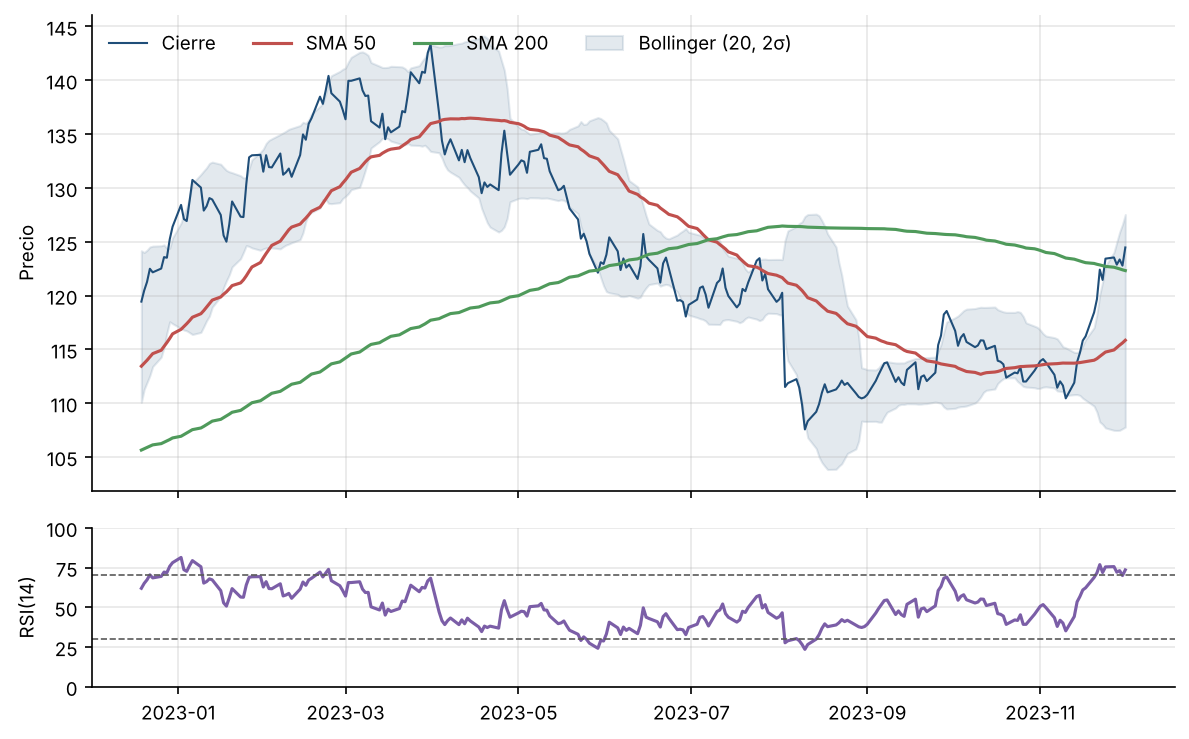
\includegraphics[width=\textwidth]{f01_indicadores}
\caption{Precio con SMA50, SMA200 y bandas de Bollinger; abajo, RSI(14) con los niveles 30/70.}
\end{figure}

\section{Volatilidad y stops: el ATR}
El rango verdadero $TR_t = \max(H_t-L_t,\ |H_t-C_{t-1}|,\ |L_t-C_{t-1}|)$ incluye los gaps; su media de
Wilder es el ATR. Colocar el stop a $k\cdot\text{ATR}$ ($k=1{,}5$--$3$) adapta la distancia al ruido del
activo y, combinado con el tamaño por riesgo (capítulo~\ref{cap:riesgo}), hace que cada operación
arriesgue lo mismo en dinero aunque los activos tengan volatilidades muy diferentes.

\section{Niveles}
\begin{itemize}
\item \textbf{Máximos y mínimos previos} (día, semana, 20 sesiones): donde se acumulan stops y órdenes.
\item \textbf{Canal de Donchian}: máximo y mínimo de las $n$ sesiones \emph{anteriores}. Romperlo es la
  base de los sistemas de seguimiento de tendencia tipo «tortuga» (\py{trader.backtest.donchian\_breakout}).
\item \textbf{Pivotes clásicos} (\py{trader.indicators.pivot\_points}) a partir del H, L, C de la sesión
  previa: $P=(H+L+C)/3$, $R_1=2P-L$, $S_1=2P-H$, $R_2=P+(H-L)$, $S_2=P-(H-L)$. Útiles intradía como
  referencias que mucha gente mira.
\item \textbf{VWAP} de la sesión: referencia de los algoritmos institucionales.
\end{itemize}

\begin{aviso}[El técnico no es una ventaja por sí mismo]
Cualquier regla técnica debe pasar por el proceso del capítulo~\ref{cap:backtest}. Un indicador sirve
para \emph{estructurar} la decisión (régimen, nivel, stop), no para sustituir una hipótesis de por qué
el precio debería moverse.
\end{aviso}

\begin{ejercicios}
\begin{enumerate}
\item Calcula los pivotes con $H=110$, $L=90$, $C=100$ y compáralos con la salida de \py{pivot\_points}.
\item Ejecuta \py{python scripts/backtest.py --estrategia rsi} y luego con \py{--estrategia sma}. ¿Cuál
  tiene más operaciones? ¿Cuál es más sensible a los costes (\py{--coste 5})?
\end{enumerate}
\end{ejercicios}

\chapter{Gestión del riesgo y tamaño de posición}\label{cap:riesgo}

\begin{clave}[La regla más importante del curso]
Decide \textbf{cuánto puedes perder} antes de decidir cuánto puedes ganar. El tamaño de la posición se
calcula a partir del stop, no al revés.
\end{clave}

\section{Riesgo por operación y múltiplos de R}
Define $1R$ como el dinero que pierdes si salta el stop. Todo se mide en $R$: una operación que gana
$3R$ ganó tres veces lo arriesgado. Los profesionales arriesgan típicamente entre el 0,25~\% y el 1~\%
del capital por operación; rara vez más del 2~\%.

\section{Tamaño por stop}\label{sec:tamano}
Con capital $C$, riesgo $\rho$ (fracción), entrada $E$, stop $S$ y valor del punto $v$ (dinero por
unidad de precio y de tamaño):
\begin{equation}\label{eq:tamano}
N = \left\lfloor \frac{\rho\, C}{|E-S|\, v}\right\rfloor .
\end{equation}
\begin{table}[h]\centering\small
\begin{tabular}{lll}
\toprule
Mercado & Valor del punto $v$ & Función \\ \midrule
Acciones & 1 por acción & \py{risk.position\_size\_stop} \\
FX & valor del pip por lote $/$ tamaño del pip & \py{fx.pip\_value}, \py{fx.lots\_for\_risk} \\
Futuros & multiplicador del contrato (CL: 1000~\$) & \py{commodities.futures\_position\_size} \\
Stop por ATR & $|E-S| = k\cdot\text{ATR}$ & \py{risk.atr\_position\_size} \\
\bottomrule
\end{tabular}
\end{table}

\paragraph{Ejemplo.} Capital 50\,000~€, riesgo 0,5~\% (250~€), compra a 182,40 con stop en 176,90:
$N=\lfloor 250/5{,}50\rfloor = 45$ acciones. El nocional (8208~€) es solo el 16~\% del capital: el
riesgo lo fija el stop, no el nocional.
\begin{lstlisting}
python scripts/tamano_posicion.py accion --capital 50000 --riesgo 0.5 --entrada 182.4 --stop 176.9 --objetivo 195
\end{lstlisting}

\section{Volatility targeting}
En carteras y estrategias sistemáticas el tamaño se fija para que cada posición aporte una
volatilidad objetivo $\sigma^*$:
\begin{equation}
w_t = \min\!\left(\frac{\sigma^*}{\hat\sigma_t},\ L_{\max}\right),
\end{equation}
con $\hat\sigma_t$ estimada solo con datos hasta $t$ (\py{risk.vol\_target\_weight},
\py{backtest.vol\_targeted}). Reduce exposición cuando el mercado se agita, que es cuando suelen llegar
las pérdidas grandes.

\section{Kelly: cuánto arriesgar}
Si en cada apuesta ganas $b$ veces lo arriesgado con probabilidad $p$ y pierdes lo arriesgado con
probabilidad $1-p$, apostando una fracción $f$ del capital el crecimiento logarítmico esperado es
\begin{equation}
g(f) = p\ln(1+fb) + (1-p)\ln(1-f),
\end{equation}
que se maximiza en la \textbf{fracción de Kelly}
\begin{equation}\label{eq:kelly}
f^* = p - \frac{1-p}{b}\qquad\left(\text{continuo: } f^*=\frac{\mu}{\sigma^2}\right).
\end{equation}
\begin{figure}[h]\centering
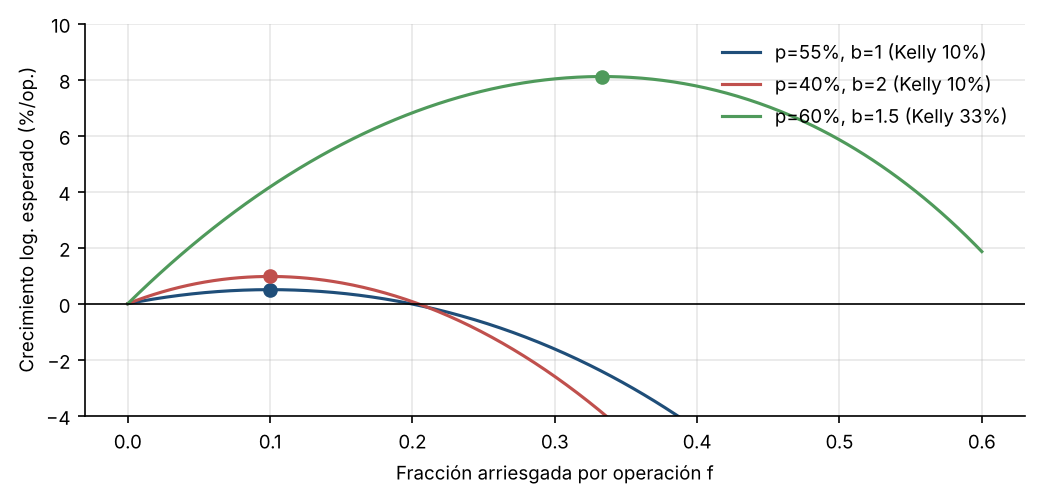
\includegraphics[width=0.85\textwidth]{f03_kelly}
\caption{Crecimiento esperado frente a la fracción arriesgada. Pasado Kelly el crecimiento cae y a
$2f^*$ es aproximadamente nulo: arriesgar de más destruye riqueza aunque la ventaja sea real.}
\label{fig:kelly}
\end{figure}

\begin{aviso}[Nunca uses Kelly completo]
$p$ y $b$ son estimaciones con mucho error. Sobrestimar la ventaja te lleva a la zona de la derecha de
la figura~\ref{fig:kelly}. Los profesionales usan entre $1/4$ y $1/2$ de Kelly, que sacrifica poco
crecimiento (con $f^*/2$ se obtiene en torno al 75~\% del crecimiento máximo) y reduce mucho la volatilidad.
\end{aviso}

\section{Riesgo de ruina y drawdown}
El drawdown es la caída desde el máximo previo, $DD_t = E_t/\max_{s\le t}E_s - 1$
(\py{risk.drawdown}). Recuperar una caída exige una subida mayor: tras perder un 50~\% hay que ganar
un 100~\%. La figura~\ref{fig:ruina} (Monte Carlo, \py{risk.risk\_of\_ruin\_mc}) muestra que la
probabilidad de sufrir un drawdown del 30~\% se dispara con el riesgo por operación, incluso con
ventaja real.
\begin{figure}[h]\centering
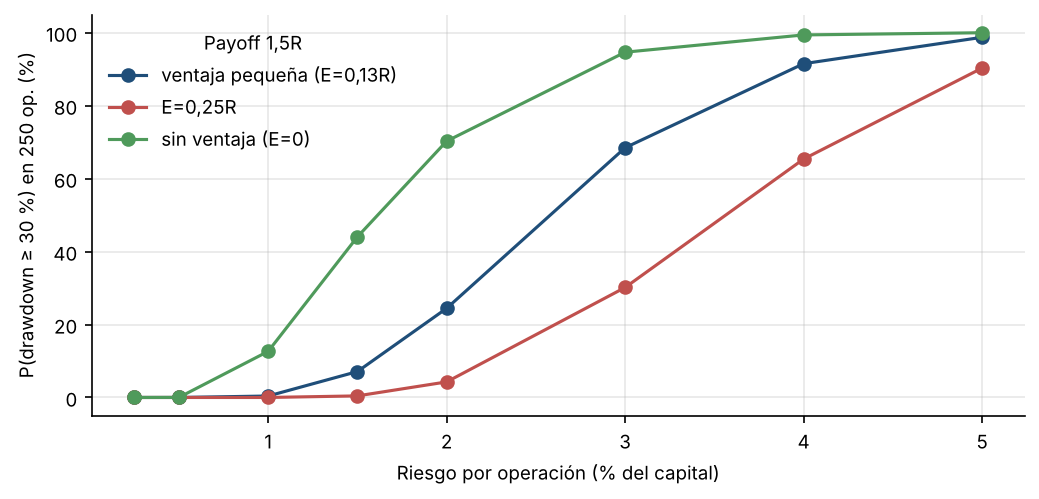
\includegraphics[width=0.85\textwidth]{f04_ruina}
\caption{Probabilidad de un drawdown $\ge 30~\%$ en 250 operaciones según el riesgo por operación.}
\label{fig:ruina}
\end{figure}

Con 10 pérdidas seguidas (algo frecuente con un 40~\% de acierto: $0{,}6^{10}\approx0{,}6~\%$ por
cada tramo de 10, pero en cientos de operaciones es casi seguro que ocurra alguna racha así), arriesgar
un 1~\% cuesta un 9,6~\%; arriesgar un 5~\% cuesta un 40~\%.

\section{Medidas de riesgo de cartera}
\paragraph{VaR y Expected Shortfall.} El VaR al nivel $\alpha$ es la pérdida que solo se supera con
probabilidad $1-\alpha$; el ES es la pérdida media \emph{cuando} se supera. Bajo normalidad
\begin{equation}
\text{VaR}_\alpha = -\mu - \sigma\,\Phi^{-1}(1-\alpha),\qquad
\text{ES}_\alpha = -\mu + \sigma\,\frac{\varphi(\Phi^{-1}(\alpha))}{1-\alpha}.
\end{equation}
Con $\mu=0$: VaR$_{99}=2{,}33\sigma$ y ES$_{97,5}=2{,}34\sigma$ (por eso Basilea usa ES al 97,5~\%).
La versión histórica usa los cuantiles empíricos (\py{risk.var\_historical}, \py{es\_historical}).

\paragraph{Contribuciones al riesgo.} Con pesos (o nocionales) $w$ y covarianza $\Sigma$,
$\sigma_p=\sqrt{w^\top\Sigma w}$ y la contribución de cada posición es
\begin{equation}
RC_i = \frac{w_i (\Sigma w)_i}{\sigma_p},\qquad \sum_i RC_i = \sigma_p .
\end{equation}
Una posición pequeña pero muy correlacionada con el resto puede dominar el riesgo.
\py{scripts/informe\_riesgo.py} muestra la tabla de contribuciones, VaR/ES y un estrés común.

\section{Límites de una mesa profesional}
\begin{itemize}
\item \textbf{Pérdida diaria máxima} (p.~ej. 2--3~\% del capital o 3R): al tocarla, se deja de operar ese día.
\item \textbf{Drawdown máximo} (p.~ej. 10~\%): al tocarlo, se reduce el tamaño a la mitad hasta recuperar.
\item \textbf{Riesgo abierto total}: suma de las distancias a los stops $\le$ 4--6~\% del capital.
\item \textbf{Concentración}: límites por activo, sector, divisa y factor.
\item \textbf{Apalancamiento bruto} y \textbf{liquidez}: no tener más de un 10--20~\% del volumen diario.
\end{itemize}

\begin{ejercicios}
\begin{enumerate}
\item Con $p=0{,}45$ y $b=2$, calcula Kelly y medio Kelly. Comprueba con \py{risk.growth\_rate} que medio Kelly da aproximadamente el 75~\% del crecimiento.
\item Tu sistema tiene un 35~\% de acierto. ¿Qué probabilidad hay de 8 pérdidas consecutivas en una secuencia concreta de 8? Simula cuántas rachas así aparecen en 500 operaciones.
\item Ejecuta \py{scripts/informe\_riesgo.py} y explica por qué el VaR histórico al 99~\% difiere del normal.
\end{enumerate}
\end{ejercicios}

\chapter{Evaluación de estrategias y backtesting}\label{cap:backtest}

\section{Métricas}
Con rentabilidades por periodo $r_t$ y $P$ periodos por año:
\begin{align*}
\text{CAGR} &= \Big(\prod_t (1+r_t)\Big)^{P/n}-1, &
\text{Sharpe} &= \sqrt{P}\,\frac{\overline{r - r_f}}{s(r)}, \\
\text{Sortino} &= \sqrt{P}\,\frac{\overline{r-r_f}}{\sqrt{\E[\min(r,0)^2]}}, &
\text{Calmar} &= \frac{\text{CAGR}}{|\text{Max DD}|}.
\end{align*}
Por operación (\py{performance.trade\_stats}): tasa de acierto, \emph{payoff} (ganancia media / pérdida
media), \emph{profit factor} (suma de ganancias / suma de pérdidas) y esperanza (ec.~\ref{eq:esperanza}).

\paragraph{Sharpe probabilístico (PSR).} El Sharpe estimado tiene error, que crece con la asimetría
negativa y la curtosis. Bailey y López de Prado (2012) proponen
\begin{equation}
\text{PSR}(SR^*) = \Phi\!\left(\frac{(\widehat{SR}-SR^*)\sqrt{n-1}}{\sqrt{1-\gamma_3\widehat{SR}+\frac{\gamma_4-1}{4}\widehat{SR}^2}}\right),
\end{equation}
con $\widehat{SR}$ por periodo (sin anualizar), $\gamma_3$ la asimetría y $\gamma_4$ la curtosis
(\py{performance.probabilistic\_sharpe}). Exige PSR $>0{,}95$ antes de creerte un Sharpe.

\section{El backtest vectorizado sin mirar al futuro}
La regla de oro: la posición decidida con información hasta el cierre de $t$ solo puede ganar o perder
con la rentabilidad de $t$ a $t+1$:
\begin{equation}
\pi_t = q_{t-1}\, r_t - c\,|q_t - q_{t-1}| ,
\end{equation}
con $q$ la posición y $c$ el coste por unidad de rotación. Es exactamente lo que hace
\py{trader.backtest.backtest} (y un test lo vigila).

\begin{figure}[h]\centering
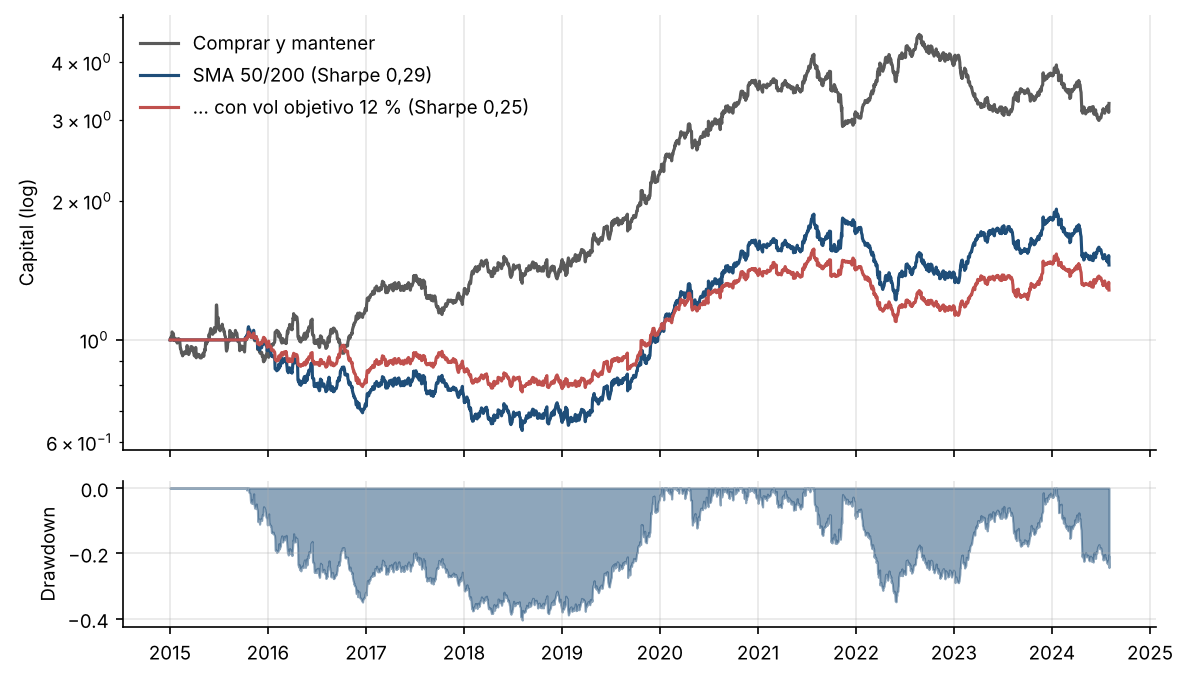
\includegraphics[width=0.95\textwidth]{f05_backtest}
\caption{Cruce de medias 50/200 sobre datos sintéticos, con y sin volatility targeting, y su drawdown.
En un activo con deriva positiva, el seguimiento de tendencia suele quedarse por detrás de comprar y
mantener: lo que aporta es reducir los drawdowns largos, no batir al activo.}
\end{figure}

\section{Los sesgos que destruyen backtests}
\begin{description}
\item[Look-ahead.] Usar información que no se tenía: cierres para decidir en la apertura del mismo día,
  datos fundamentales antes de su publicación, máximos del día en curso.
\item[Supervivencia.] Probar solo con las acciones que existen hoy olvida las que quebraron.
\item[Costes irreales.] Ignorar spread, comisiones, impacto, préstamo de títulos para cortos o el coste
  de financiación del apalancamiento.
\item[Sobreajuste (data snooping).] Probar muchas variantes y quedarse con la mejor.
\end{description}

\section{Sobreajuste: el sesgo de selección}\label{sec:sobreajuste}
Si pruebas $N$ configuraciones \emph{sin ventaja alguna}, el mejor Sharpe in-sample crece como
\begin{equation}
\E[\max_N \widehat{SR}] \approx \sigma_{SR}\Big[(1-\gamma)\Phi^{-1}\!\big(1-\tfrac1N\big)+\gamma\,\Phi^{-1}\!\big(1-\tfrac{1}{Ne}\big)\Big],
\end{equation}
con $\gamma\approx0{,}5772$ (\py{performance.expected\_max\_sharpe}). Con 3 años de datos
($\sigma_{SR}\approx 1/\sqrt{3}$), probar 100 variantes produce un «Sharpe 1,5» de puro ruido
(figura~\ref{fig:sobreajuste}).
\begin{figure}[h]\centering
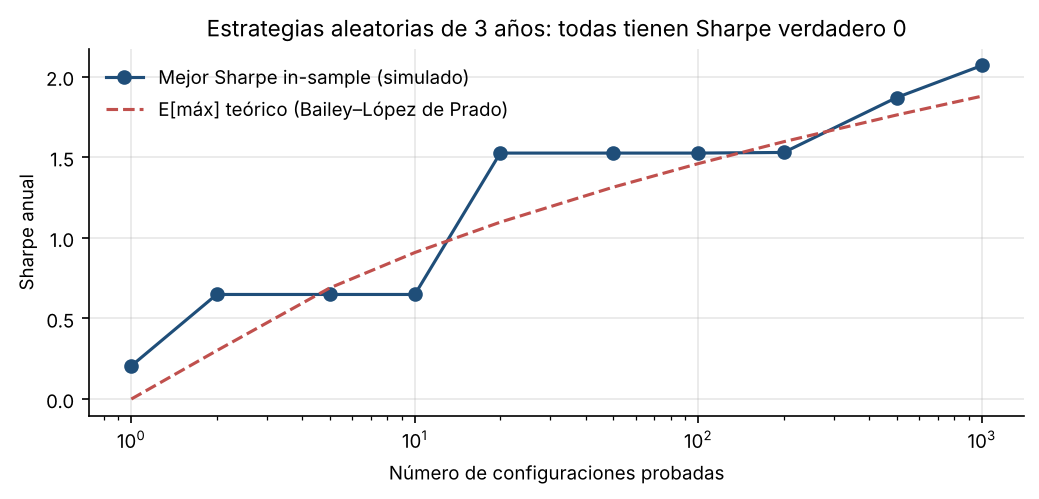
\includegraphics[width=0.85\textwidth]{f06_sobreajuste}
\caption{El mejor Sharpe de $N$ estrategias aleatorias. Si no cuentas cuántas pruebas hiciste, no sabes
lo que vale tu mejor resultado.}\label{fig:sobreajuste}
\end{figure}

\begin{practica}[Protocolo mínimo]
\begin{enumerate}
\item Escribe la hipótesis económica \emph{antes} de mirar los datos: ¿quién pierde el dinero que vas a ganar y por qué?
\item Reserva un tramo final de datos que no tocarás hasta el final (\emph{hold-out}).
\item Usa pocos parámetros y valores redondos; comprueba que los vecinos del óptimo también funcionan (meseta, no pico).
\item Valida en \emph{walk-forward} (\py{backtest.walk\_forward\_splits}): optimiza en una ventana, prueba en la siguiente.
\item Duplica los costes. Prueba en otros activos y otros periodos.
\item Anota cuántas variantes probaste y exige un Sharpe por encima del máximo esperado por azar.
\item Opera primero en papel o con tamaño mínimo y compara con el backtest.
\end{enumerate}
\end{practica}

\begin{ejercicios}
\begin{enumerate}
\item Con \py{scripts/backtest.py} prueba todas las combinaciones de \py{--rapida} 10, 20, 50 y \py{--lenta} 100, 150, 200. Anota el mejor Sharpe y compáralo con \py{expected\_max\_sharpe(9, ...)}.
\item Introduce a propósito un look-ahead (quita el \py{shift(1)} en una copia de \py{backtest}) y observa cómo «mejora» el resultado.
\end{enumerate}
\end{ejercicios}

\chapter{Psicología, proceso y diario de trading}\label{cap:psico}

\section{Sesgos que cuestan dinero}
\begin{description}
\item[Aversión a la pérdida y efecto disposición.] Vendemos rápido lo que gana y aguantamos lo que
  pierde. Es exactamente lo contrario de «cortar pérdidas y dejar correr beneficios». Solución: stop y
  objetivo definidos antes de entrar; mover el stop solo a favor.
\item[Exceso de confianza.] Tras una racha ganadora se aumenta el tamaño. El tamaño lo fija la regla, no el ánimo.
\item[Revenge trading.] Operar para «recuperar» una pérdida. Solución: límite de pérdida diaria que obliga a parar.
\item[Sesgo de confirmación.] Buscar solo noticias que apoyan la posición. Escribe qué te haría cambiar de opinión.
\item[Sesgo de resultado.] Juzgar una decisión por su resultado. Una buena operación puede perder dinero; una mala puede ganarlo.
\item[FOMO.] Entrar tarde en un movimiento ya hecho, con el stop lejos y la relación beneficio/riesgo destruida.
\end{description}

\section{El plan de trading}
Un plan escrito responde, para cada \emph{setup}:
\begin{enumerate}
\item \textbf{Contexto}: régimen, mercado, horario en que se opera.
\item \textbf{Disparador}: condición exacta de entrada.
\item \textbf{Invalidación}: dónde está el stop y por qué (nivel que demuestra que la idea era errónea).
\item \textbf{Tamaño}: ec.~\eqref{eq:tamano} con el riesgo fijado.
\item \textbf{Gestión}: objetivo, salida parcial, stop dinámico (ATR, mínimos crecientes), salida por tiempo.
\item \textbf{Qué no hacer}: no operar en noticias de primer nivel si el setup no lo contempla, etc.
\end{enumerate}

\section{El diario de operaciones}
El diario es el \emph{dataset} más valioso del trader. Cada operación registra fecha, activo, lado,
entrada, stop, salida, tamaño, comisiones, setup y notas (qué viste, cómo te sentías). Con eso se
calcula el resultado en $R$ y la esperanza por setup:
\begin{lstlisting}
python scripts/diario.py nueva --fichero diario.csv --simbolo EURUSD --clase fx --lado largo \
   --entrada 1.0850 --stop 1.0825 --salida 1.0900 --tamano 200000 --setup ruptura
python scripts/diario.py resumen --fichero diario.csv
\end{lstlisting}
El resumen marca las operaciones que perdieron más de $1{,}2R$ (stops saltados o movidos, el error más
caro y más corregible). Revisa el diario cada semana: elimina los setups con esperanza negativa tras
30--50 operaciones y aumenta el peso de los que funcionan.

\begin{clave}
El objetivo no es acertar, es \textbf{ejecutar el proceso}. Puntúa cada día por cumplimiento del plan
(0--10), no por P\&L. A largo plazo el P\&L sigue al proceso.
\end{clave}

\section{Hábitos}
Sueño, ejercicio y pausas no son consejos de autoayuda: la fatiga deteriora la toma de decisiones bajo
riesgo. Define un horario de trabajo, no mires la cuenta fuera de él y para tras dos errores de
disciplina en un mismo día.

\part{Clases de activo}
\chapter{Renta variable (Equity)}\label{cap:equity}

\section{El mercado}
Se negocian acciones individuales, índices (vía futuros como ES/NQ/FESX, ETFs como SPY/QQQ, o CFD),
sectores y opciones. Rasgos propios:
\begin{itemize}
\item \textbf{Deriva positiva a largo plazo} (prima de riesgo de la renta variable de 4--6~\% anual): ir
  corto es nadar contra corriente y requiere pedir prestado el título (coste de préstamo, riesgo de
  \emph{recall} y de \emph{short squeeze}).
\item \textbf{Eventos corporativos}: resultados trimestrales (gaps de $\pm5$--$15~\%$), dividendos,
  ampliaciones, splits, OPAs. El calendario de resultados es imprescindible.
\item \textbf{Asimetría de volatilidad}: las caídas son más rápidas y volátiles que las subidas; la
  volatilidad implícita (VIX) sube cuando el mercado baja.
\item \textbf{Fuerte factor común}: la mayoría de las acciones tienen beta positiva con el índice.
\end{itemize}

\section{Beta, CAPM y alfa}
La beta mide la sensibilidad al mercado:
\begin{equation}
\beta_i = \frac{\operatorname{Cov}(r_i,r_m)}{\operatorname{Var}(r_m)},\qquad
r_i - r_f = \alpha + \beta_i(r_m-r_f)+\varepsilon .
\end{equation}
(\py{equity.beta}, \py{equity.capm}). Una cartera de 10 acciones de beta 1,4 es, en gran parte, una
apuesta apalancada al índice. Para aislar la idea específica (\emph{alfa}) se cubre la beta vendiendo
$\beta\cdot$nocional del futuro del índice.

\paragraph{Factores.} Más allá del mercado, las rentabilidades se explican por factores como tamaño
(SMB), valor (HML), momentum (12--1 meses), calidad/rentabilidad y baja volatilidad.
\py{equity.factor\_regression} estima la exposición de una estrategia a factores; si tu «alfa»
desaparece al añadir el momentum, no tenías alfa, tenías momentum.

\paragraph{Momentum 12--1.} Rentabilidad de los últimos 12 meses excluyendo el último
(\py{equity.momentum\_12\_1}); el último mes muestra reversión a corto plazo.

\section{Setups habituales}
\begin{description}
\item[Ruptura con volumen.] Salida de un rango tras compresión de volatilidad, con volumen relativo
  alto. Stop bajo el rango; funciona mejor en régimen alcista del índice.
\item[Pullback en tendencia.] Retroceso a la media de 20/50 en una acción líder (fuerza relativa alta).
\item[Gap tras resultados.] Los gaps con sorpresa de beneficios grande tienden a continuar (\emph{post-earnings
  announcement drift}); los gaps sin noticia en acciones grandes tienden a cerrarse más
  (\py{equity.gap\_stats} mide la tasa de cierre).
\item[Reversión a corto plazo.] RSI(2) extremo en acciones/índices en tendencia alcista.
\end{description}

\section{Trading de pares (valor relativo)}
Dos acciones con el mismo negocio (KO/PEP, bancos de un mismo país) pueden estar
\textbf{cointegradas}: aunque cada precio es un paseo aleatorio, una combinación es estacionaria.
\begin{enumerate}
\item Estimar $\beta$ en $\ln y_t = a + \beta\ln x_t + s_t$ \emph{con datos pasados} (\py{equity.hedge\_ratio}).
\item Contrastar estacionariedad del spread $s_t$ (Dickey--Fuller, \py{equity.adf\_tstat}; con $\beta$
  estimado el crítico al 5~\% es $\approx -3{,}34$).
\item Vida media de reversión del AR(1) $\Delta s_t = a + b\,s_{t-1}$: $HL = -\ln 2/\ln(1+b)$
  (\py{equity.half\_life}). Debe ser corta frente al horizonte de la operación.
\item Operar el $z$-score: vender el spread si $z>2$, comprarlo si $z<-2$, cerrar si $|z|<0{,}5$
  (\py{equity.pair\_positions}).
\end{enumerate}
\begin{figure}[h]\centering
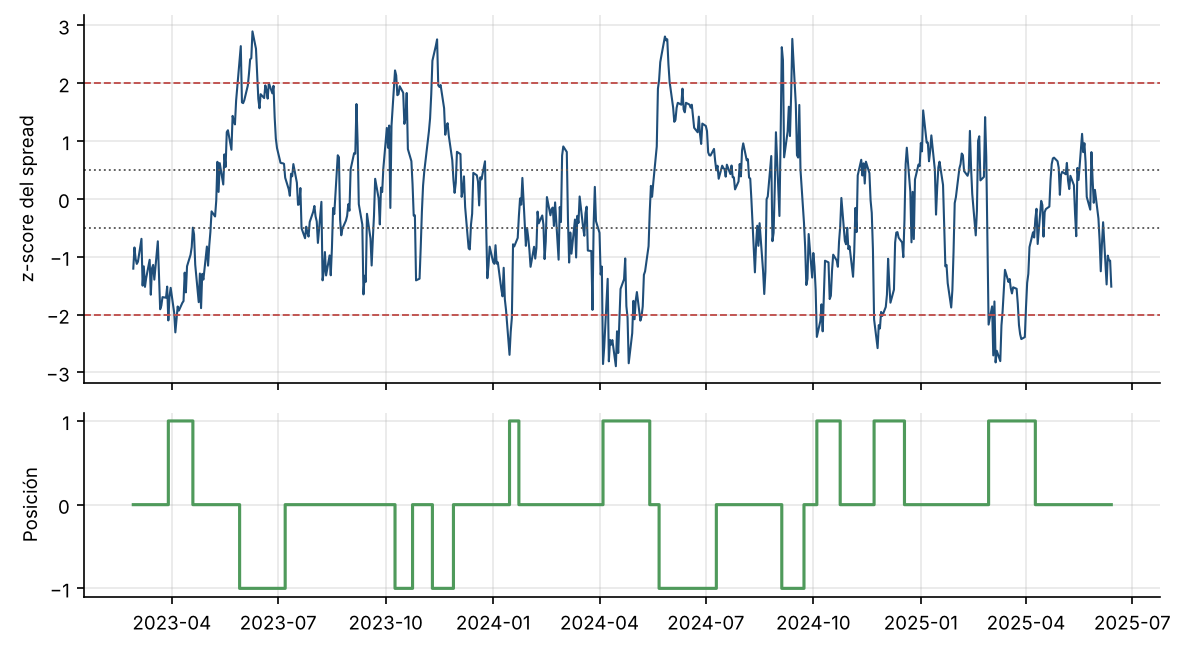
\includegraphics[width=0.9\textwidth]{f07_pares}
\caption{$z$-score de un spread cointegrado (fuera de la muestra de estimación de $\beta$) y la posición resultante.}
\end{figure}
\begin{aviso}
La cointegración se rompe (OPAs, cambios de negocio, crisis). Pon siempre un stop en $z$ (p.~ej. $|z|>4$)
y en tiempo (3--4 vidas medias).
\end{aviso}

\begin{ejercicios}
\begin{enumerate}
\item Calcula la beta de una acción con \py{equity.capm} sobre tus datos. ¿Cuántos contratos de futuro
  del índice cubren una cartera de 500\,000~\$ con beta 1,2 si el futuro tiene nocional 250\,000~\$?
\item Ejecuta \py{python scripts/backtest.py --estrategia pares} y relaciona la vida media con la duración de las operaciones.
\end{enumerate}
\end{ejercicios}

\chapter{Divisas (FX)}\label{cap:fx}

\section{Convenciones}
Un par \texttt{BASE/COTIZADA} indica cuántas unidades de la cotizada vale una de la base:
EURUSD $=1{,}0850$ significa 1~EUR $=1{,}0850$~USD. Comprar el par es comprar la base y vender la
cotizada. Mayores: EURUSD, USDJPY, GBPUSD, USDCHF, AUDUSD, USDCAD, NZDUSD; el resto son cruces.

\begin{itemize}
\item \textbf{Pip}: 0,0001 (0,01 si la cotizada es JPY) — \py{fx.pip\_size}.
\item \textbf{Lote estándar}: 100\,000 unidades de la base (mini 10\,000, micro 1000).
\item \textbf{Valor del pip} por lote: $0{,}0001\times100\,000=10$ unidades de la cotizada; se convierte
  a la divisa de la cuenta (\py{fx.pip\_value}). En EURUSD con cuenta en USD vale 10~\$; en USDJPY a
  150, $1000/150=6{,}67$~\$.
\end{itemize}

\begin{lstlisting}
python scripts/tamano_posicion.py fx --capital 20000 --riesgo 1 --par EURUSD --tipo 1.0850 --stop-pips 25
\end{lstlisting}

\paragraph{Tipos cruzados.} EURJPY $=$ EURUSD $\times$ USDJPY; EURGBP $=$ EURUSD $/$ GBPUSD. En general,
pasando por USD (\py{fx.cross\_rate}). Si el cruce cotizado se desvía del implícito más que los
spreads, hay arbitraje triangular (\py{fx.triangular\_arbitrage}); en la práctica solo lo capturan los
creadores de mercado más rápidos.

\section{Forwards y paridad cubierta de intereses}
No arbitraje entre invertir en cotizada o cambiar, invertir en base y cerrar con un forward:
\begin{equation}\label{eq:cip}
F = S\,\frac{1+r_{\text{cot}}\,T}{1+r_{\text{base}}\,T}\quad(\text{convención monetaria, } T=\text{días}/360).
\end{equation}
Los \textbf{puntos forward} son $(F-S)/\text{pip}$ (\py{fx.forward\_rate}, \py{fx.forward\_points}). La
divisa con tipo de interés más alto cotiza con \emph{descuento} a plazo.

\section{Carry trade}
Comprar la divisa de tipo alto financiándose en la de tipo bajo cobra el diferencial de tipos:
\begin{equation}
\text{rent.} = \frac{(1+r_b T)S_1 - (1+r_q T)S_0}{S_0} \approx \frac{S_1}{S_0}-1 + (r_b-r_q)T
\end{equation}
(\py{fx.carry\_return}). La paridad \emph{no cubierta} diría que la divisa de tipo alto se deprecia lo
justo para anular el carry; empíricamente no lo hace en promedio (\emph{forward premium puzzle}), y por
eso el carry ha sido rentable\ldots{} con \textbf{asimetría negativa}: sube por la escalera y baja por
el ascensor (1998, 2008, agosto de 2024 con el yen).
\begin{figure}[h]\centering
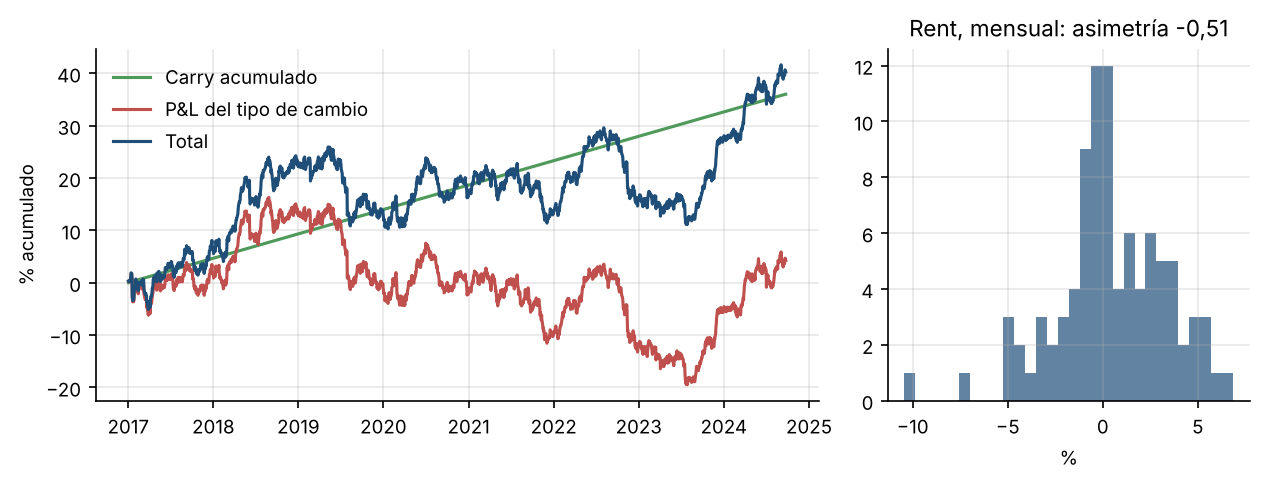
\includegraphics[width=\textwidth]{f08_carry}
\caption{Carry trade simulado: el diferencial se acumula de forma estable, pero el tipo de cambio sufre
caídas bruscas que generan una distribución mensual con cola izquierda.}
\end{figure}

\section{Qué mueve las divisas}
\begin{itemize}
\item \textbf{Diferenciales de tipos reales y expectativas de bancos centrales}: el factor dominante a
  medio plazo. Sigue los tipos a 2 años de cada país y el calendario de reuniones (Fed, BCE, BoJ, BoE).
\item \textbf{Datos macro}: empleo (NFP), IPC, PMI, PIB. El movimiento depende de la sorpresa frente al consenso.
\item \textbf{Aversión al riesgo}: USD, JPY y CHF suelen apreciarse en crisis; AUD, NZD y emergentes depreciarse.
\item \textbf{Términos de intercambio}: CAD y NOK con el petróleo, AUD con el mineral de hierro y China.
\item \textbf{Valor a largo plazo}: la paridad de poder adquisitivo relativa
  $S_{\text{justo}} = S_0\,\frac{P_{q,t}/P_{q,0}}{P_{b,t}/P_{b,0}}$ (\py{fx.relative\_ppp}) es un ancla débil a varios años.
\item \textbf{Flujos e intervenciones}: fixing de fin de mes, repatriaciones, intervenciones (BoJ, SNB).
\end{itemize}

\begin{practica}
En FX el tamaño se piensa en pips de stop y en lotes. Calcula siempre el valor del pip en la divisa de
tu cuenta y vigila la \textbf{correlación} entre pares: largo EURUSD y largo GBPUSD es,
principalmente, una sola apuesta corta en dólares. Ten en cuenta el \emph{swap} nocturno (el carry) que
cobra o paga tu broker y los spreads amplios en la apertura de Sídney y en noticias.
\end{practica}

\begin{ejercicios}
\begin{enumerate}
\item EURUSD $=1{,}0850$, tipo USD 4,5~\%, tipo EUR 2,25~\%. Calcula el forward a 90 días y los puntos
  (\py{python scripts/calculadoras.py forward ...}).
\item Valor del pip de EURGBP para una cuenta en USD con GBPUSD $=1{,}27$.
\item ¿Por qué un carry trade financiado en yenes sufre cuando sube la volatilidad global?
\end{enumerate}
\end{ejercicios}

\chapter{Materias primas (Commodities)}\label{cap:commodities}

\section{Futuros: el instrumento}
Las materias primas se operan casi siempre con \textbf{futuros}: contratos estandarizados con
vencimiento, tamaño y entrega definidos. Lo que hay que conocer de cada contrato:
\begin{table}[h]\centering\small
\begin{tabular}{llllr}
\toprule
Símbolo & Contrato & Cotiza en & Multiplicador & Valor del tick \\ \midrule
CL & WTI (NYMEX) & \$/bbl & 1000 bbl & 10~\$ (0,01) \\
BZ & Brent (ICE) & \$/bbl & 1000 bbl & 10~\$ (0,01) \\
NG & Gas natural & \$/MMBtu & 10\,000 MMBtu & 10~\$ (0,001) \\
RB / HO & Gasolina / gasóleo & \$/gal & 42\,000 gal & 4,20~\$ (0,0001) \\
GC & Oro (COMEX) & \$/oz & 100 oz & 10~\$ (0,10) \\
SI & Plata & \$/oz & 5000 oz & 25~\$ (0,005) \\
HG & Cobre & \$/lb & 25\,000 lb & 12,50~\$ (0,0005) \\
ZC / ZS / ZW & Maíz / soja / trigo & ¢/bu & 5000 bu & 12,50~\$ (1/4 ¢) \\
\bottomrule
\end{tabular}
\caption{Especificaciones (\py{commodities.CONTRACTS}). Códigos de mes: F G H J K M N Q U V X Z = ene--dic.}
\end{table}

Un movimiento de 1~\$ en el crudo son 1000~\$ por contrato. Con un stop de 1,60~\$ y un riesgo de
1875~\$ solo cabe un contrato (\py{futures\_position\_size}); si no cabe ninguno, existen
micro-contratos (MCL, MGC) de 1/10.

\section{La curva de futuros}
El modelo de coste de mantenimiento (\emph{cost of carry}) relaciona contado y futuro:
\begin{equation}\label{eq:carry}
F(T) = S\,e^{(r+u-y)T},
\end{equation}
con $r$ el tipo de interés, $u$ el coste de almacenamiento y $y$ el \textbf{rendimiento de
conveniencia} (el valor de tener el físico disponible). Despejando,
$y = r+u-\ln(F/S)/T$ (\py{implied\_convenience\_yield}).
\begin{itemize}
\item \textbf{Contango} (curva creciente): inventarios abundantes, almacenaje caro. Típico de oro (casi
  puro coste financiero) y de gas en verano.
\item \textbf{Backwardation} (curva decreciente): escasez; el físico hoy vale más que mañana.
\end{itemize}

\section{Roll yield: por qué el precio no es la rentabilidad}
Quien mantiene exposición tiene que \emph{rodar} el contrato antes del vencimiento: vender el que vence
y comprar el siguiente. Si la curva no cambia, el contrato va «subiendo» o «bajando» por la curva hacia
el contado. El roll yield anualizado entre dos vencimientos es
\begin{equation}
RY = \frac{\ln(F_{\text{cerca}}/F_{\text{lejos}})}{T_{\text{lejos}}-T_{\text{cerca}}}
\end{equation}
(\py{commodities.roll\_yield}, \py{roll\_yield\_curve}): positivo en backwardation, negativo en contango.
\begin{figure}[h]\centering
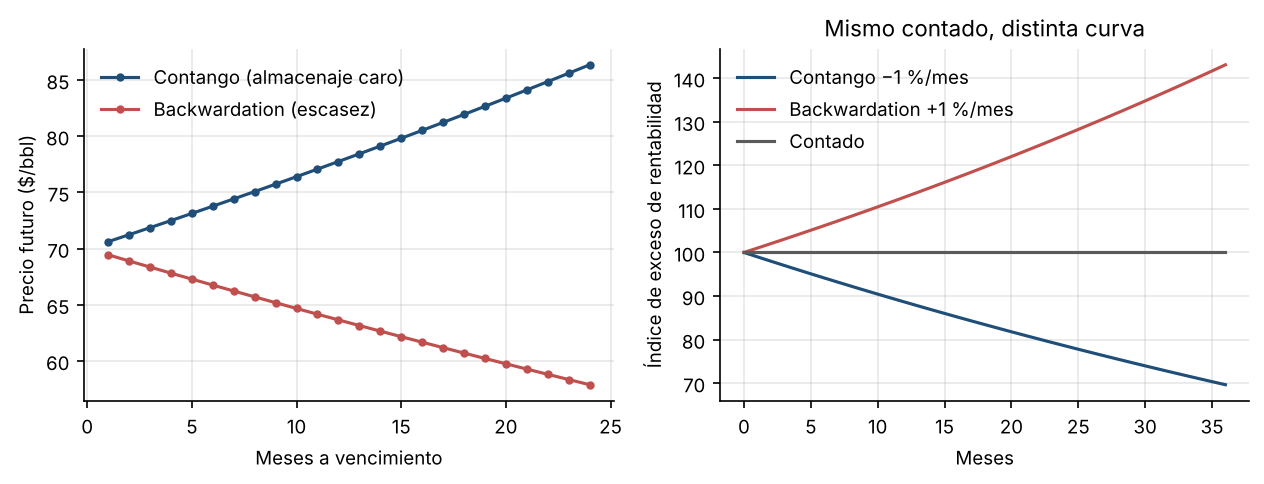
\includegraphics[width=\textwidth]{f09_curvas}
\caption{Izquierda: curvas en contango y backwardation. Derecha: con el mismo precio de contado, un
inversor que rueda gana o pierde un 1~\% mensual según la forma de la curva.}
\end{figure}
\begin{aviso}
Los ETF de materias primas que ruedan futuros en contango (gas natural, VIX) pierden valor de forma
sistemática aunque el contado no se mueva. Y las series «continuas» que enlazan contratos sin ajustar
tienen saltos falsos en cada roll: usa series ajustadas por ratio (\py{ratio\_back\_adjust}) para
backtests.
\end{aviso}

\paragraph{Carry como señal.} Estar largo en las materias primas con mayor backwardation y corto en las de
mayor contango (estrategia de \emph{carry} o de estructura de curva) es una de las primas más
documentadas del sector.

\section{Spreads}
Los traders de materias primas operan mucho más spreads que direcciones:
\begin{itemize}
\item \textbf{Calendario}: largo un vencimiento, corto otro (apuesta a la forma de la curva).
\item \textbf{Crack 3:2:1} (margen de refino, \$/bbl): $\big(2\cdot\text{RB}\cdot42+\text{HO}\cdot42-3\cdot\text{CL}\big)/3$ (\py{crack\_spread\_321}).
\item \textbf{Crush} de soja (\$/bu): harina$\times0{,}022$ + aceite$\times0{,}11$ $-$ soja (\py{crush\_spread}).
\item \textbf{Spark spread} (\$/MWh): electricidad $-$ heat rate $\times$ gas (\py{spark\_spread}).
\item \textbf{Inter-mercado}: Brent--WTI, oro/plata, trigo/maíz.
\end{itemize}

\section{Fundamentales y calendario}
\begin{itemize}
\item \textbf{Energía}: inventarios semanales EIA (miércoles, crudo; jueves, gas), reuniones de la OPEP+,
  huracanes, informes AIE. Margen de refino y estacionalidad (gasolina en verano, gasóleo en invierno).
\item \textbf{Metales preciosos}: tipos reales (el oro cae cuando suben los tipos reales a 10 años) y
  dólar; compras de bancos centrales; plata y platino con componente industrial.
\item \textbf{Metales industriales}: ciclo industrial y China (PMI), inventarios LME/SHFE.
\item \textbf{Agrícolas}: informes USDA (WASDE mensual, siembras de marzo, acreage de junio), clima,
  estacionalidad de cosecha (\py{monthly\_seasonality}).
\item \textbf{Posicionamiento}: informe COT de la CFTC (viernes): posiciones especulativas extremas
  anticipan giros.
\end{itemize}

\begin{practica}
Nunca mantengas un futuro con entrega física hasta el primer día de aviso (\emph{first notice day})
si no puedes recibir el físico: rueda antes. El 20 de abril de 2020 el WTI de mayo cotizó a $-37$~\$
porque los compradores sin almacenaje no podían recibir el crudo.
\end{practica}

\begin{ejercicios}
\begin{enumerate}
\item Precios CL 78,1 / 77,4 / 76,9 / 76,5 para 1--4 meses: forma de la curva y roll yield
  (\py{python scripts/calculadoras.py curva --precios ... --meses 1 2 3 4}).
\item Crudo 75~\$, RBOB 2,35~\$/gal, HO 2,55~\$/gal: calcula el crack 3:2:1.
\item Con oro a 2400~\$, tipo 4,5~\% y futuro a 6 meses a 2460~\$, ¿qué rendimiento de conveniencia
  implícito hay (con $u=0$)?
\end{enumerate}
\end{ejercicios}

\chapter{Renta fija y tipos de interés}\label{cap:rates}

Todos los mercados dependen de los tipos: descuentan los flujos de las acciones, determinan el carry de
las divisas y el coste de mantener materias primas. Un trader de cualquier mesa debe saber leer la
curva de tipos y medir el riesgo de tipo de interés.

\section{Precio, TIR y curva}
Un bono de nominal $N$, cupón anual $c$, $f$ pagos al año y TIR $y$:
\begin{equation}
P = \sum_{k=1}^{fT}\frac{CF_k}{(1+y/f)^{k}},\qquad CF_k = \tfrac{cN}{f}\ (+N \text{ al final})
\end{equation}
(\py{rates.bond\_price}, \py{rates.ytm}). Precio y TIR se mueven en sentido contrario. Si $y=c$ el bono
cotiza a la par. La \textbf{curva} (TIR frente a plazo) suele tener pendiente positiva; su inversión
(2 años por encima de 10 años) ha precedido a la mayoría de las recesiones de EE.~UU.

\section{Duración, convexidad y DV01}
\begin{align}
D_{\text{mac}} &= \frac{\sum t_k\,CF_k\,d_k}{P}, &
D_{\text{mod}} &= \frac{D_{\text{mac}}}{1+y/f} = -\frac1P\frac{dP}{dy},\\
C &= \frac1P\frac{d^2P}{dy^2}, &
\text{DV01} &= D_{\text{mod}}\cdot P\cdot 0{,}0001 .
\end{align}
\begin{equation}
\Delta P \approx -D_{\text{mod}}\,P\,\Delta y + \tfrac12\,C\,P\,(\Delta y)^2 .
\end{equation}
\begin{figure}[h]\centering
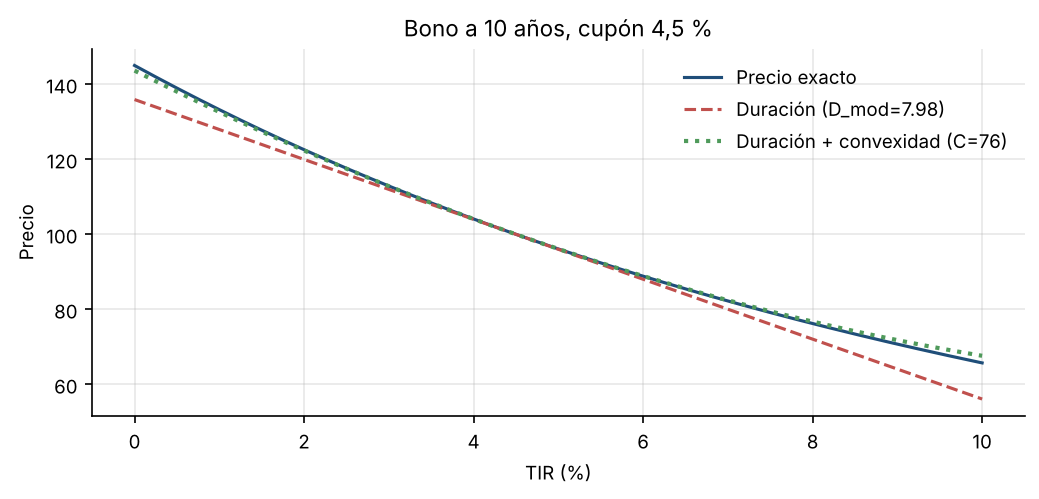
\includegraphics[width=0.85\textwidth]{f10_bono}
\caption{Precio frente a TIR: la duración es la tangente; la convexidad corrige la curvatura.}
\end{figure}
El DV01 (o PV01) es la unidad de riesgo de una mesa de tipos: cuánto se gana o pierde por cada punto
básico. Un bono a 10 años con DV01 de 0,080 por 100 de nominal arriesga unos 800~\$ por pb por cada
millón.
\begin{lstlisting}
python scripts/calculadoras.py bono --cupon 4.25 --tir 4.4 --anos 10
\end{lstlisting}

\section{Operaciones típicas}
\begin{itemize}
\item \textbf{Direccional}: largo duración si esperas bajadas de tipos (con futuros: ZN, ZB, Bund FGBL).
\item \textbf{Pendiente} (\emph{steepener}/\emph{flattener}): largo 2 años y corto 10 años (o al revés) con
  \textbf{DV01 neutro}, de modo que un desplazamiento paralelo no afecta: nocional de cobertura
  $=$ DV01$_{\text{posición}}/$DV01$_{\text{cobertura}}$ (\py{rates.dv01\_hedge\_ratio}).
\item \textbf{Mariposa}: 2s5s10s, apuesta a la curvatura.
\item \textbf{Carry y roll-down}: con curva positiva, un bono a 5 años se convierte en uno a 4,75 años
  y su TIR «rueda» hacia abajo por la curva, generando rentabilidad si la curva no cambia.
\end{itemize}

\begin{ejercicios}
\begin{enumerate}
\item Comprueba numéricamente que $D_{\text{mac}}$ de un bono cupón cero es su vencimiento.
\item Tienes 10 millones de un bono a 2 años con DV01 0,019 por 100. ¿Cuánto nominal del 10 años
  (DV01 0,080) vendes para un steepener DV01 neutro?
\end{enumerate}
\end{ejercicios}

\chapter{Opciones y volatilidad}\label{cap:opciones}

\section{Black--Scholes y sus variantes}
Para una call europea con dividendo continuo $q$:
\begin{equation}
C = S e^{-qT}N(d_1) - K e^{-rT}N(d_2),\qquad d_{1,2}=\frac{\ln(S/K)+(r-q\pm\frac12\sigma^2)T}{\sigma\sqrt T},
\end{equation}
y la paridad put--call $C-P = Se^{-qT}-Ke^{-rT}$ (\py{options.bs\_price}). La misma fórmula cubre las tres clases de activo:
\begin{itemize}
\item \textbf{Acciones/índices}: $q$ = rentabilidad por dividendo.
\item \textbf{FX} (Garman--Kohlhagen): $q = r_{\text{extranjero}}$ (\py{garman\_kohlhagen}).
\item \textbf{Futuros de materias primas} (Black-76): $S=F$, $q=r$ (\py{black76}).
\end{itemize}

\section{Griegas}
\begin{table}[h]\centering\small
\begin{tabularx}{\textwidth}{llX}
\toprule
Griega & Fórmula (call) & Significado para el trader \\ \midrule
Delta & $e^{-qT}N(d_1)$ & Equivalente en subyacente; cobertura. \\
Gamma & $e^{-qT}\varphi(d_1)/(S\sigma\sqrt T)$ & Cuánto cambia la delta: el «convexo» que se compra. \\
Vega & $Se^{-qT}\varphi(d_1)\sqrt T$ & P\&L por punto de volatilidad implícita. \\
Theta & $\partial C/\partial t$ & Lo que se paga cada día por tener gamma. \\
Rho & $KTe^{-rT}N(d_2)$ & Sensibilidad a tipos. \\
\bottomrule
\end{tabularx}
\end{table}
La relación fundamental de una cartera cubierta en delta es
\begin{equation}
\text{P\&L diario} \approx \tfrac12\,\Gamma\,S^2\left(\hat\sigma^2_{\text{realizada}}-\sigma^2_{\text{implícita}}\right)\Delta t ,
\end{equation}
es decir, \textbf{comprar opciones es apostar a que la volatilidad realizada superará a la implícita}
y venderlas, lo contrario. Esto es el núcleo del trading de volatilidad.

\begin{figure}[h]\centering
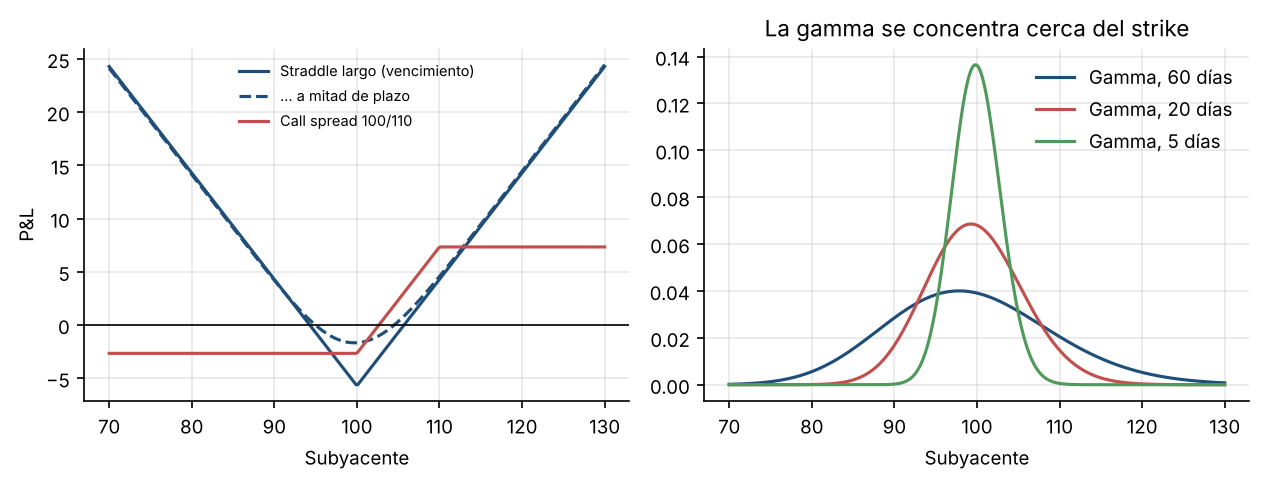
\includegraphics[width=\textwidth]{f11_opciones}
\caption{Izquierda: P\&L de un straddle largo y de un call spread. Derecha: la gamma se concentra
cerca del strike al acercarse el vencimiento.}
\end{figure}

\section{Volatilidad implícita y movimiento esperado}
La volatilidad implícita es la $\sigma$ que iguala el precio de mercado (\py{options.implied\_vol}).
El movimiento esperado a $1\sigma$ hasta una fecha es $S\,\sigma\sqrt{d/365}$
(\py{expected\_move}); el precio del straddle ATM dividido por $S$ ($\approx0{,}8\,\sigma\sqrt T$) es la
regla rápida para saber cuánto descuenta el mercado ante resultados o un dato macro.
\begin{lstlisting}
python scripts/calculadoras.py opcion --spot 100 --strike 105 --dias 30 --vol 25 --tipo-interes 4
python scripts/calculadoras.py movimiento --spot 5200 --vol 14 --dias 1
\end{lstlisting}

\paragraph{Sonrisa y estructura temporal.} En renta variable las puts bajistas tienen más volatilidad
implícita (\emph{skew}) por la demanda de protección; en FX la sonrisa es más simétrica y se cotiza en
\emph{risk reversals} y \emph{butterflies}; en materias primas a menudo el skew es alcista (miedo a
subidas de oferta escasa). La prima de varianza (implícita $>$ realizada en promedio) es la razón por la
que vender volatilidad es rentable\ldots{} con colas izquierdas muy gruesas (febrero de 2018).

\section{Estrategias básicas}
\begin{itemize}
\item \textbf{Call/put largas}: direccionales con pérdida acotada.
\item \textbf{Spreads verticales}: abaratan la prima a cambio de limitar la ganancia.
\item \textbf{Straddle/strangle}: largo volatilidad (comprado) o corto volatilidad (vendido).
\item \textbf{Covered call / cash-secured put}: venta de volatilidad sobre una posición o un objetivo de compra.
\item \textbf{Collar}: protección financiada vendiendo potencial alcista.
\item \textbf{Calendarios}: apuesta a la estructura temporal.
\end{itemize}

\begin{ejercicios}
\begin{enumerate}
\item Verifica la paridad put--call con \py{bs\_price} para varios strikes.
\item Una acción a 100 tiene el straddle ATM de 7 días a 5,60. ¿Qué movimiento descuenta el mercado? ¿Qué volatilidad implícita aproximada supone?
\end{enumerate}
\end{ejercicios}

\chapter{Cripto: perpetuos, funding y base}\label{cap:cripto}

Las criptomonedas se negocian 24/7, con volatilidades de 50--80~\% anual y correlación creciente con
los activos de riesgo. El instrumento dominante es el \textbf{futuro perpetuo}: no vence y se ancla al
contado mediante un pago periódico entre largos y cortos, el \emph{funding}.
\begin{itemize}
\item Si el perpetuo cotiza por encima del contado, el funding es positivo: \textbf{los largos pagan a
  los cortos}. Funding anualizado $= \text{tasa}\times(24/8)\times365$ (\py{crypto.annualized\_funding}):
  un 0,01~\% cada 8 horas son casi un 11~\% anual.
\item Futuros con vencimiento: base anualizada $(F/S-1)\cdot365/d$ (\py{annualized\_basis}).
\item \textbf{Cash and carry}: comprar contado y vender futuro captura la base (\py{cash\_and\_carry\_pnl})
  con riesgo de contraparte y de margen en la pata corta.
\end{itemize}

\paragraph{Liquidación.} Con apalancamiento $L$ en margen aislado, la liquidación de un largo llega
aproximadamente en $E(1-1/L+mm)$ (\py{crypto.liquidation\_price}). Con 20x, un movimiento del 5~\% en
contra liquida la posición. La regla del curso aplica igual: el tamaño se fija por el stop, y la
liquidación debe quedar \emph{mucho} más lejos que el stop (el script \py{tamano\_posicion.py cripto}
avisa si no es así).

\begin{aviso}
Riesgos propios: contraparte (quiebras de plataformas), custodia, cascadas de liquidaciones en fines de
semana con poca liquidez, manipulación en activos pequeños y regulación cambiante. Diversifica
plataformas y no dejes en ellas más capital del que necesitas como margen.
\end{aviso}

\part{Práctica diaria}
\chapter{La rutina diaria con los scripts}\label{cap:rutina}

\section{Antes de la sesión (30--45 min)}
\begin{enumerate}
\item \textbf{Calendario}: datos macro con hora y consenso, bancos centrales, resultados de empresas,
  inventarios (EIA), vencimientos de opciones y futuros.
\item \textbf{Contexto}: qué hicieron Asia y Europa, futuros de índices, dólar, bonos a 10 años, crudo,
  oro, VIX. ¿Régimen de riesgo (\emph{risk-on}) o de aversión (\emph{risk-off})?
\item \textbf{Hoja premercado}: niveles, volatilidad y régimen de tu lista de seguimiento.
\begin{lstlisting}
python scripts/premercado.py --csv datos/SPY.csv --csv datos/EURUSD.csv --csv datos/CL.csv
\end{lstlisting}
  Imprime el checklist, las sesiones FX abiertas, ATR, volatilidad, RSI, distancia a las medias,
  pivotes, máximos/mínimos de 20 sesiones y el rango esperado del día.
\item \textbf{Escenarios si/entonces}: «si rompe 1,0900 con volumen tras el IPC, compro con stop 1,0870».
\item \textbf{Riesgo}: revisa el riesgo abierto y la cartera.
\begin{lstlisting}
python scripts/informe_riesgo.py --csv datos/cartera.csv --pos SPY=50000 --pos TLT=-20000 --pos GLD=15000
\end{lstlisting}
\end{enumerate}

\section{Durante la sesión}
\begin{itemize}
\item Calcula el tamaño \emph{antes} de enviar la orden:
\begin{lstlisting}
python scripts/tamano_posicion.py futuro --capital 250000 --riesgo 0.75 --simbolo CL --entrada 74.2 --stop 72.6
python scripts/tamano_posicion.py fx --capital 20000 --par USDJPY --tipo 151.2 --stop-pips 40
\end{lstlisting}
\item Envía stop y objetivo con la entrada (orden bracket).
\item Calculadoras rápidas: opciones, IV, movimiento esperado, forward, cruces, curva, crack, bonos, funding
  (\py{scripts/calculadoras.py --help}).
\item Respeta el límite de pérdida diaria.
\end{itemize}

\section{Después de la sesión}
\begin{enumerate}
\item Anota cada operación en el diario (\py{scripts/diario.py nueva}).
\item Puntúa el cumplimiento del plan del día.
\item Semanalmente: \py{scripts/diario.py resumen}, revisión de setups y de errores.
\item Mensualmente: re-evalúa estrategias sistemáticas con \py{scripts/backtest.py} y compara el
  resultado real con el esperado.
\end{enumerate}

\section{Datos}
Los scripts leen CSV con columna de fecha y \texttt{open, high, low, close[, volume]} (o una columna por
activo para el informe de riesgo). Puedes exportarlos desde tu bróker o plataforma; si instalas
\texttt{yfinance}, \py{trader.data.download("SPY")} descarga históricos diarios. Sin
\texttt{--csv}, todo funciona con datos sintéticos para practicar.

\section{Mapa de scripts}
\begin{table}[h]\centering\small
\begin{tabularx}{\textwidth}{lX}
\toprule
Script & Para qué \\ \midrule
\py{premercado.py} & Checklist, sesiones FX, niveles y régimen de cada activo. \\
\py{tamano\_posicion.py} & Tamaño por riesgo: acciones, FX, futuros, ATR, cripto (con aviso de liquidación). \\
\py{informe\_riesgo.py} & Vol, VaR/ES, contribuciones, correlaciones y estrés de la cartera. \\
\py{backtest.py} & Backtest de SMA, Donchian, RSI y pares con costes, métricas y gráfico. \\
\py{diario.py} & Diario de operaciones en CSV y estadísticas en $R$ por setup. \\
\py{calculadoras.py} & Opciones, IV, movimiento esperado, forward FX, cruces, curva, crack, bonos, funding. \\
\py{generar\_figuras.py} & Regenera las figuras de este PDF. \\
\bottomrule
\end{tabularx}
\end{table}

\chapter{Plan de estudio de 12 semanas}\label{cap:plan}

\begin{table}[h]\centering\small
\begin{tabularx}{\textwidth}{clX}
\toprule
Semana & Tema & Tarea práctica \\ \midrule
1 & Caps.~\ref{cap:intro}--\ref{cap:micro} & Abre una cuenta demo. Ejecuta todos los scripts en modo demo. Mide spreads de 5 activos. \\
2 & Cap.~\ref{cap:estadistica} & Descarga 10 años de 3 activos de clases distintas: volatilidad, colas, correlaciones. \\
3 & Cap.~\ref{cap:tecnico} & Ejecuta \py{premercado.py} cada día con tus CSV. Escribe escenarios si/entonces. \\
4 & Cap.~\ref{cap:riesgo} & Define por escrito tus límites (riesgo/op., pérdida diaria, drawdown). Simula la ruina con tus números. \\
5 & Cap.~\ref{cap:backtest} & Backtest de una idea con el protocolo completo y hold-out. Cuenta las variantes probadas. \\
6 & Cap.~\ref{cap:psico} & Escribe el plan de trading de 2 setups. Empieza el diario (también en demo). \\
7 & Cap.~\ref{cap:equity} & Beta y factores de tu lista; estudia un par cointegrado. \\
8 & Cap.~\ref{cap:fx} & Calcula valor del pip, forwards y carry de 5 pares; sigue un dato NFP/IPC en directo. \\
9 & Cap.~\ref{cap:commodities} & Curvas de CL, NG y GC; roll yield; sigue el informe EIA. \\
10 & Caps.~\ref{cap:rates}--\ref{cap:opciones} & DV01 de un steepener; movimiento esperado antes de resultados frente al real. \\
11 & Cap.~\ref{cap:cripto} + repaso & Funding y base; repaso del diario: esperanza por setup. \\
12 & Cap.~\ref{cap:rutina} & Rutina completa durante 5 días seguidos. Decide si pasar a tamaño real mínimo. \\
\bottomrule
\end{tabularx}
\end{table}

\begin{clave}[Criterio para pasar a dinero real]
Al menos 50 operaciones en demo siguiendo el plan, esperanza positiva en $R$ tras costes, ninguna
pérdida mayor de $1{,}5R$ por stops movidos y respeto del límite diario el 100~\% de los días. Empieza
con el tamaño mínimo posible: el objetivo de los primeros meses es comprobar que tu ejecución real se
parece a la de la demo, no ganar dinero.
\end{clave}

\part{Ampliaciones}
\chapter{Signaturas de caminos: el orden de los movimientos}\label{cap:signaturas}

Los indicadores clásicos resumen una serie con niveles (medias, máximos, volatilidad). La
\textbf{signatura} de un camino, que viene de la teoría de \emph{rough paths} de T.~Lyons, resume
también el \emph{orden} en que se mueven varias series a la vez. En investigación cuantitativa se usa
como fuente de rasgos para modelos lineales, para medir qué activo se mueve antes y para problemas de
ejecución. Este capítulo es una ampliación opcional: explica qué es, qué propiedades tiene de verdad
(en particular, qué significa que sea «invariante» y qué no) y la implementa en
\py{trader.signature}. Las demostraciones están en la guía teórica del repositorio (capítulo de rough
paths) y en las referencias de la bibliografía.

\section{Motivación: dos caminos con las mismas rentabilidades}
Supón dos activos A y B que suben un 1~\% cada uno en una sesión. En el camino~1 sube primero A y
después B; en el camino~2, al revés. El incremento total es idéntico, la volatilidad también, y una
estrategia que mire sólo rentabilidades de cierre a cierre no distingue los dos casos. Sin embargo, si A
se mueve sistemáticamente antes que B, eso es información operable (y un riesgo si estás cubriendo B
con A). La signatura es una forma sistemática de capturar ese orden.

\section{Definición y cálculo}
Sea $X:[0,T]\to\mathbb R^d$ un camino (por ejemplo, $d$ log-precios). Su signatura es la sucesión de
integrales iteradas
\begin{equation}\label{eq:signatura}
S^{i}=\int_0^T dX^i_s,\qquad
S^{ij}=\iint_{0<s<u<T} dX^i_s\,dX^j_u,\qquad
S^{ijk}=\iiint_{0<s<u<v<T} dX^i_s\,dX^j_u\,dX^k_v,\ \dots
\end{equation}
El nivel~1 son los incrementos; el nivel~2 contiene, además de productos de incrementos, el
\emph{área de Lévy} $A^{ij}=\tfrac12(S^{ij}-S^{ji})$; el nivel~3 añade información sobre el orden de
tres movimientos. Truncada en el nivel $m$, tiene $d+d^2+\dots+d^m$ términos.

\paragraph{Cálculo exacto con datos discretos.} Se unen los datos con segmentos rectos. Para un único
segmento de incremento $\Delta$, la signatura es la exponencial tensorial:
$(\Delta,\ \tfrac12\Delta^{\otimes2},\ \tfrac16\Delta^{\otimes3})$. Para concatenar dos tramos se usa la
\textbf{identidad de Chen}: $S(X\ast Y)=S(X)\otimes S(Y)$, es decir,
\begin{equation}\label{eq:chen}
S^{(2)}(X\ast Y)=S^{(2)}(X)+S^{(1)}(X)\otimes S^{(1)}(Y)+S^{(2)}(Y),
\end{equation}
y análogamente en el nivel~3. Con incrementos $\Delta_k$ y sumas previas $C_k=\sum_{j<k}\Delta_j$ queda
$S^{(2)}=\sum_k\big(C_k\otimes\Delta_k+\tfrac12\Delta_k^{\otimes2}\big)$, que \py{signature.signature}
calcula vectorizado sobre lotes de caminos o ventanas.

\paragraph{Identidad de barajado.} Los productos de términos de la signatura son combinaciones lineales
de términos de nivel superior; en el nivel~2, $S^iS^j=S^{ij}+S^{ji}$. Por eso la parte simétrica de
$S^{(2)}$ no aporta nada nuevo: $S^{(2)}=\tfrac12 S^{(1)}\otimes S^{(1)}+A$, y la
\emph{log-signatura} de nivel~2 es simplemente $(S^{(1)},A)$ (\py{signature.log\_signature2}). Esta
propiedad hace que una función \emph{lineal} de la signatura sea muy expresiva: con el tiempo como
canal adicional, cualquier función continua del camino se aproxima tan bien como se quiera por funciones
lineales de la signatura truncada (\emph{universalidad}).

\section{Invarianzas: qué ve y qué no ve la signatura}
\paragraph{Reparametrización.} Si $\varphi$ es un cambio de reloj creciente, el camino $X\circ\varphi$
recorre los mismos puntos a otra velocidad, y
\begin{equation}
S(X\circ\varphi)=S(X).
\end{equation}
Para datos de mercado esto significa que pausas, ticks repetidos, muestreo irregular o un ritmo de
llegada variable \emph{del mismo camino} no cambian los rasgos. Es la propiedad a la que se refiere la
expresión «invarianza frente a la latencia»: si una fuente de datos entrega los mismos precios en el
mismo orden pero con retrasos variables, la signatura de cada serie es la misma. Además, la signatura
es invariante por traslación (no depende del nivel de partida) y, salvo tramos que se deshacen sobre sí
mismos, determina el camino (Hambly y Lyons, 2010).

\begin{table}[h]\centering\small
\begin{tabularx}{\textwidth}{Xll}
\toprule
Cambio en los datos & ¿Cambia la signatura? & Comentario \\ \midrule
Pausas, ticks repetidos, ritmo de llegada & No & reparametrización \\
Subdividir un tramo recto & No & reparametrización \\
Sumar una constante a los precios & No & traslación \\
Retraso de un activo respecto a otro & \textbf{Sí} & lo mide el área de Lévy (\S\ref{sec:levy}) \\
Movimiento rápido frente a lento, con canal de tiempo & \textbf{Sí} & \py{signature.add\_time} \\
Perder puntos intermedios (muestreo más grueso) & \textbf{Sí}, en general & otro camino lineal a trozos \\
Latencia de tus órdenes & No aplica & es un coste de ejecución \\
\bottomrule
\end{tabularx}
\caption{Lo que la signatura ignora y lo que no (comprobado en \py{tests/test\_signature.py}).}
\end{table}

\begin{aviso}[La signatura no hace inmune a la latencia]
La invarianza es una propiedad de los \emph{rasgos}, no de la estrategia. Si tus órdenes llegan tarde
pagas el deslizamiento igual (capítulo~\ref{cap:micro}). Y un retraso \emph{relativo} entre dos activos
no se ignora: aparece en el área de Lévy, lo que es útil para detectarlo pero también puede crear
señales falsas si los dos activos cierran a horas distintas. Por último, ignorar el ritmo tiene un
coste: la velocidad del mercado (volatilidad por unidad de tiempo) importa, y para recuperarla hay que
añadir el tiempo como canal, con lo que se pierde la invarianza.
\end{aviso}

\section{Transformación lead-lag y variación cuadrática}
La signatura de un solo canal no ve la volatilidad: $S^{11}=\tfrac12(S^1)^2$ depende sólo del
incremento. La \textbf{transformación lead-lag} (\py{signature.lead\_lag}) duplica la serie en una
copia adelantada y otra retrasada: primero se mueve la adelantada y luego la retrasada la alcanza
(figura~\ref{fig:signaturas}, izquierda). El área de Lévy entre ambas copias es exactamente la mitad
de la variación cuadrática:
\begin{equation}\label{eq:leadlag}
A^{\text{lead},\text{lag}}=\tfrac12\sum_k(\Delta x_k)^2 .
\end{equation}
Así la varianza realizada aparece en el nivel~2 sin calcularla a mano, y los niveles superiores capturan
momentos de orden mayor y su relación con la dirección del precio.

\section{Área de Lévy: quién se mueve primero}\label{sec:levy}
Para dos canales, $A^{12}=\tfrac12\int(X^1\,dX^2-X^2\,dX^1)$ es el área con signo entre el camino y la
cuerda que une sus extremos: si se recorre un cuadrado unidad en sentido antihorario, $A^{12}=1$. Si
$X^1$ sube y \emph{después} sube $X^2$, el área es positiva; si es al revés, negativa. Por eso
$A^{12}>0$ indica que el canal~1 tiende a moverse antes.

Calculada sobre todo el histórico, el área es muy ruidosa (su desviación típica crece como la propia
señal). \py{signature.lead\_lag\_score} estandariza las rentabilidades, las acumula en ventanas sin
solape de $w$ sesiones y promedia el área normalizada por $(w-1)/2$. Su esperanza es
\begin{equation}\label{eq:score}
\E[\text{puntuación}]=\sum_{h=1}^{w-1}\frac{w-h}{w-1}\big[\rho_{x\to y}(h)-\rho_{y\to x}(h)\big],
\qquad \rho_{x\to y}(h)=\operatorname{corr}(r^x_t,r^y_{t+h}),
\end{equation}
que se reduce a $\rho_{x\to y}(1)-\rho_{y\to x}(1)$ si sólo hay desfase de un periodo. El error típico
sale de la dispersión entre ventanas. La figura~\ref{fig:signaturas} (derecha) lo comprueba con
$r^B_t=\rho\,r^A_{t-1}+\sqrt{1-\rho^2}\,\varepsilon_t$: la puntuación estimada sigue la recta $\rho$.
\begin{lstlisting}
python scripts/calculadoras.py liderazgo --csv datos/cierres.csv --a SPY --b EWJ
\end{lstlisting}

\begin{figure}[h]\centering
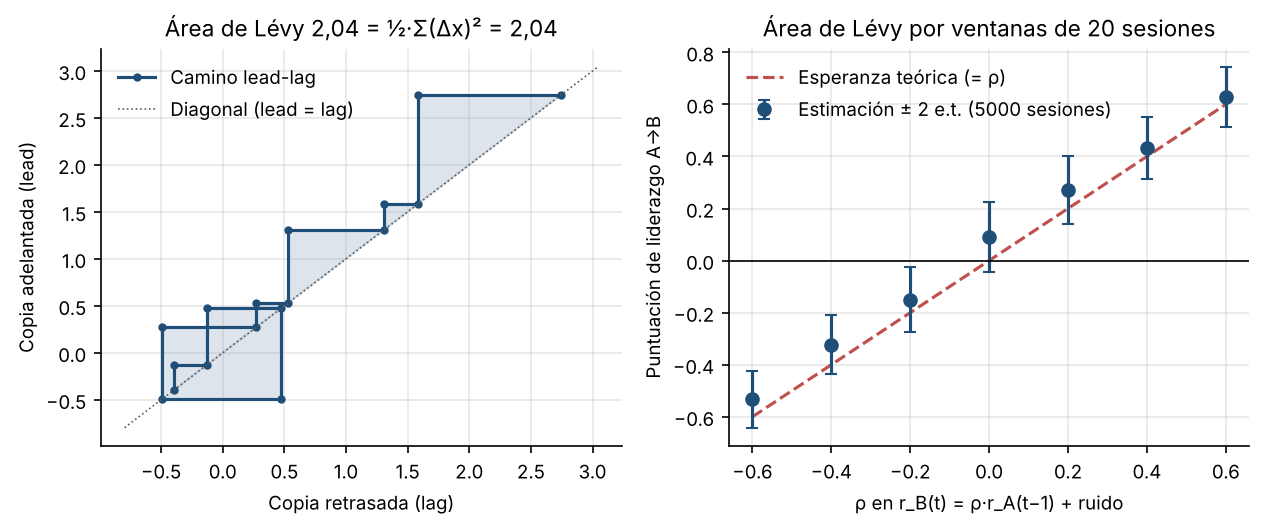
\includegraphics[width=\textwidth]{f12_signaturas}
\caption{Izquierda: camino lead-lag de 9 precios; el área sombreada es la mitad de la variación
cuadrática~\eqref{eq:leadlag}. Derecha: puntuación de liderazgo~\eqref{eq:score} frente al valor teórico.}
\label{fig:signaturas}
\end{figure}

\begin{practica}[Cierres asíncronos]
Con cierres diarios, un mercado que cierra antes (Tokio) parece «seguir» a uno que cierra después
(Nueva York) el día anterior: es un artefacto del horario, no una ventaja. Lo mismo ocurre con activos
poco líquidos cuyo último precio es antiguo (\emph{precios rancios}), que además hacen que la correlación
medida baje al aumentar la frecuencia (efecto Epps). Antes de operar un liderazgo, compruébalo con
precios tomados a la misma hora y descuenta costes: los desfases que se ven en datos diarios suelen
estar ya arbitrados en datos intradía. Para covarianzas con datos asíncronos, el estimador de
Hayashi--Yoshida es la referencia.
\end{practica}

\section{Una estrategia lineal sobre la signatura}
\py{signature.window\_features} construye, para cada sesión y con datos sólo hasta ella, el camino de
la ventana de $w$ sesiones: tiempo, log-precio relativo dividido por la volatilidad de la ventana y su
transformación lead-lag. Se calcula la signatura (nivel~2: 10 rasgos; nivel~3: 36, una vez quitados los
términos de tiempo puro, que son constantes). \py{signature.sig\_momentum} (y
\py{backtest.signature\_momentum}) ajusta una regresión \emph{ridge} de la rentabilidad del día
siguiente sobre esos rasgos, con reestimación walk-forward (capítulo~\ref{cap:backtest}): cada $63$
sesiones se reajusta con las $500$ anteriores cuyo resultado ya se conoce, y la posición es el signo de
la predicción.
\begin{lstlisting}
python scripts/backtest.py --estrategia sig --ventana 20 --coste 2
\end{lstlisting}
Los tests comprueban que no hay look-ahead, que con rentabilidades autocorrelacionadas (AR(1) con
$\phi=0{,}3$) la estrategia gana fuera de muestra y, por el script, que sobre un paseo aleatorio no
encuentra ventaja: con los datos sintéticos por defecto su Sharpe es negativo, como debe ser.

\paragraph{Extensiones en la literatura.} Futter, Horvath y Wiese (2023) formulan la cartera de
media-varianza con señales exógenas como un funcional lineal de la signatura y obtienen la solución
explícita en función de la signatura esperada. Kalsi, Lyons y Pérez Arribas (2020) resuelven la
ejecución óptima buscando la velocidad de negociación entre funciones lineales de la signatura.

\section{Límites}
\begin{itemize}
\item \textbf{Dimensión.} Con $d$ canales y nivel $m$ hay $\sim d^m$ rasgos: con 5 activos y nivel~3,
  155. Sin regularización (ridge, lasso) y validación fuera de muestra, el sobreajuste está
  garantizado (capítulo~\ref{cap:backtest}).
\item \textbf{Interpolación.} Con datos discretos la signatura depende de cómo se unan los puntos
  (lineal, lead-lag, escalonado). Elige un esquema y mantenlo.
\item \textbf{No estacionariedad.} Los rasgos son estables; la relación entre rasgos y rentabilidad
  futura, no. Reestimar y medir la degradación es obligatorio.
\item \textbf{Normalización.} Sin dividir por la escala de la ventana, los términos de nivel $m$ escalan
  como la volatilidad elevada a $m$ y dominan los regímenes volátiles.
\item \textbf{Evidencia.} La teoría es sólida; la evidencia publicada de rentabilidad fuera de muestra
  con datos reales y costes es todavía escasa. Trátalo como una herramienta de investigación.
\end{itemize}

\begin{clave}
La signatura es una forma compacta y con buena teoría de describir el \emph{orden} de los movimientos
de varias series. Ignora el ritmo al que llegan los datos de cada serie, pero sí registra el desfase
entre series; eso la hace útil para medir liderazgo y como entrada de modelos lineales regularizados.
No es una ventaja en sí misma.
\end{clave}

\begin{ejercicios}
\begin{enumerate}
\item Comprueba con \py{signature.signature} que la signatura de un camino no cambia al repetir puntos,
  y que sí cambia con \py{signature.add\_time}.
\item Calcula con \py{signature.levy\_area} el área de un rectángulo de lados 2 y 3 recorrido en
  sentido horario. ¿Qué signo tiene?
\item Ejecuta \py{calculadoras.py liderazgo} con cierres de un ETF europeo y uno estadounidense. ¿El
  resultado se mantiene si usas precios de la misma hora?
\item Compara \py{backtest.py --estrategia sig} con \py{--estrategia sma} sobre tus datos, con costes de
  2~pb, y cuenta cuántas variantes (ventana, nivel) has probado antes de quedarte con una.
\end{enumerate}
\end{ejercicios}

\appendix
\chapter{Formulario}\label{ap:formulas}
\small
\begin{tabularx}{\textwidth}{lX}
\toprule
Concepto & Fórmula · función \\ \midrule
Esperanza & $E = p\bar G-(1-p)\bar P$ · \py{performance.trade\_stats} \\
Tamaño por stop & $N=\lfloor\rho C/(|E-S|v)\rfloor$ · \py{risk.position\_size\_stop} \\
Vol targeting & $w=\min(\sigma^*/\hat\sigma, L)$ · \py{risk.vol\_target\_weight} \\
Kelly & $f^*=p-(1-p)/b$; $\mu/\sigma^2$ · \py{risk.kelly\_fraction} \\
VaR / ES normal & $-\mu-\sigma\Phi^{-1}(1-\alpha)$; $-\mu+\sigma\varphi(\Phi^{-1}(\alpha))/(1-\alpha)$ \\
Contribución al riesgo & $RC_i=w_i(\Sigma w)_i/\sigma_p$ · \py{risk.risk\_contributions} \\
Sharpe & $\sqrt P\,\bar r/s$ · \py{performance.sharpe} \\
PSR & $\Phi\big((\widehat{SR}-SR^*)\sqrt{n-1}/\sqrt{1-\gamma_3\widehat{SR}+\frac{\gamma_4-1}4\widehat{SR}^2}\big)$ \\
RSI & $100-100/(1+RS)$ · \py{indicators.rsi} \\
True range & $\max(H-L,|H-C_{-1}|,|L-C_{-1}|)$ · \py{indicators.atr} \\
Pivotes & $P=(H+L+C)/3$, $R_1=2P-L$, $S_1=2P-H$ \\
Beta & $\operatorname{Cov}(r_i,r_m)/\operatorname{Var}(r_m)$ · \py{equity.beta} \\
Vida media AR(1) & $-\ln2/\ln(1+b)$ · \py{equity.half\_life} \\
Valor del pip & $\text{pip}\cdot\text{lotes}\cdot10^5$ (en cotizada) · \py{fx.pip\_value} \\
Forward FX & $S(1+r_qT)/(1+r_bT)$ · \py{fx.forward\_rate} \\
Carry FX & $[(1+r_bT)S_1-(1+r_qT)S_0]/S_0$ · \py{fx.carry\_return} \\
Coste de carry & $F=Se^{(r+u-y)T}$ · \py{commodities.cost\_of\_carry\_forward} \\
Roll yield & $\ln(F_1/F_2)/(T_2-T_1)$ · \py{commodities.roll\_yield} \\
Crack 3:2:1 & $(2\,RB\cdot42+HO\cdot42-3\,CL)/3$ · \py{commodities.crack\_spread\_321} \\
Duración mod. & $D_{\text{mac}}/(1+y/f)$ · \py{rates.modified\_duration} \\
$\Delta P$ & $-D_{\text{mod}}P\Delta y+\frac12CP\Delta y^2$ · \py{rates.price\_change\_approx} \\
Black--Scholes & $Se^{-qT}N(d_1)-Ke^{-rT}N(d_2)$ · \py{options.bs\_price} \\
Movimiento esperado & $S\sigma\sqrt{d/365}$ · \py{options.expected\_move} \\
Funding anual & $\text{tasa}\cdot(24/h)\cdot365$ · \py{crypto.annualized\_funding} \\
Signatura nivel 2 & $S^{ij}=\sum_k (C_k^i+\tfrac12\Delta_k^i)\Delta_k^j$ · \py{signature.signature} \\
Área de Lévy & $A^{ij}=\tfrac12(S^{ij}-S^{ji})$ · \py{signature.levy\_area} \\
Área lead-lag & $\tfrac12\sum_k(\Delta x_k)^2$ · \py{signature.lead\_lag} \\
Liderazgo & $\E=\rho_{x\to y}(1)-\rho_{y\to x}(1)$ (desfase 1) · \py{signature.lead\_lag\_score} \\
\bottomrule
\end{tabularx}

\chapter{Glosario}
\small
\begin{description}
\item[Área de Lévy] Área con signo entre un camino de dos canales y su cuerda; mide cuál se mueve antes.
\item[ATR] Average True Range: volatilidad en unidades de precio.
\item[Backwardation] Curva de futuros decreciente con el vencimiento.
\item[Base] Diferencia entre contado y futuro.
\item[Bid / Ask] Mejor precio de compra / de venta en el libro.
\item[Carry] Rentabilidad que se obtiene si los precios no cambian (diferencial de tipos, roll yield, cupón).
\item[Contango] Curva de futuros creciente con el vencimiento.
\item[COT] Commitments of Traders: posiciones semanales en futuros publicadas por la CFTC.
\item[Drawdown] Caída desde el último máximo del capital.
\item[DV01] Variación del valor por 1 punto básico de tipo de interés.
\item[ES] Expected Shortfall: pérdida media más allá del VaR.
\item[First notice day] Primer día en que se puede notificar la entrega física de un futuro.
\item[Funding] Pago periódico entre largos y cortos de un perpetuo.
\item[Gamma] Sensibilidad de la delta al subyacente.
\item[Kelly] Fracción que maximiza el crecimiento logarítmico esperado.
\item[Lead-lag] Transformación que duplica una serie en copia adelantada y retrasada; su área es ½ de la variación cuadrática.
\item[Lote] 100\,000 unidades de la divisa base en FX.
\item[NFP] Non-Farm Payrolls: dato de empleo de EE.~UU.
\item[Pip] Cuarto decimal (segundo con JPY) de un tipo de cambio.
\item[R] Unidad de riesgo: la pérdida si salta el stop.
\item[Roll] Cambiar un futuro que vence por el siguiente.
\item[Sharpe] Exceso de rentabilidad por unidad de volatilidad.
\item[Signatura] Sucesión de integrales iteradas de un camino; resume el orden de los movimientos e ignora el ritmo.
\item[Slippage] Diferencia entre el precio esperado y el de ejecución.
\item[Swap (FX)] Coste o abono nocturno por mantener una posición de contado (el carry).
\item[VaR] Value at Risk: pérdida que solo se supera con probabilidad $1-\alpha$.
\item[VWAP] Precio medio ponderado por volumen.
\end{description}

\backmatter
\chapter*{Bibliografía recomendada}
\addcontentsline{toc}{chapter}{Bibliografía recomendada}
\small
\begin{itemize}
\item Bailey, D. y López de Prado, M. (2012). The Sharpe ratio efficient frontier. \emph{Journal of Risk} 15(2).
\item Bailey, D., Borwein, J., López de Prado, M. y Zhu, Q. (2014). Pseudo-mathematics and financial charlatanism. \emph{Notices of the AMS} 61(5).
\item Bayer, C., dos Reis, G., Horvath, B. y Oberhauser, H. (eds.) (2025). \emph{Signature Methods in Finance: An Introduction with Computational Applications}. Springer Finance (acceso abierto).
\item Carver, R. (2015). \emph{Systematic Trading}. Harriman House.
\item Chan, E. (2013). \emph{Algorithmic Trading: Winning Strategies and Their Rationale}. Wiley.
\item Chevyrev, I. y Kormilitzin, A. (2016). A primer on the signature method in machine learning. arXiv:1603.03788.
\item Douglas, M. (2000). \emph{Trading in the Zone}. Prentice Hall.
\item Epps, T. (1979). Comovements in stock prices in the very short run. \emph{Journal of the American Statistical Association} 74(366).
\item Fabozzi, F. (2012). \emph{Bond Markets, Analysis, and Strategies}. Pearson.
\item Futter, O., Horvath, B. y Wiese, M. (2023). Signature trading: a path-dependent extension of the mean-variance framework with exogenous signals. arXiv:2308.15135.
\item Gyurkó, L. G., Lyons, T., Kontkowski, M. y Field, J. (2013). Extracting information from the signature of a financial data stream. arXiv:1307.7244.
\item Hambly, B. y Lyons, T. (2010). Uniqueness for the signature of a path of bounded variation and the reduced path group. \emph{Annals of Mathematics} 171(1).
\item Harris, L. (2003). \emph{Trading and Exchanges: Market Microstructure for Practitioners}. Oxford University Press.
\item Hayashi, T. y Yoshida, N. (2005). On covariance estimation of non-synchronously observed diffusion processes. \emph{Bernoulli} 11(2).
\item Hull, J. (2021). \emph{Options, Futures, and Other Derivatives}, 11.ª ed. Pearson.
\item Ilmanen, A. (2011). \emph{Expected Returns}. Wiley.
\item Kalsi, J., Lyons, T. y Pérez Arribas, I. (2020). Optimal execution with rough path signatures. \emph{SIAM Journal on Financial Mathematics} 11(2).
\item Koijen, R., Moskowitz, T., Pedersen, L. y Vrugt, E. (2018). Carry. \emph{Journal of Financial Economics} 127(2).
\item López de Prado, M. (2018). \emph{Advances in Financial Machine Learning}. Wiley.
\item Lyons, T. (1998). Differential equations driven by rough signals. \emph{Revista Matemática Iberoamericana} 14(2).
\item Moskowitz, T., Ooi, Y. H. y Pedersen, L. (2012). Time series momentum. \emph{Journal of Financial Economics} 104(2).
\item Natenberg, S. (2014). \emph{Option Volatility and Pricing}, 2.ª ed. McGraw-Hill.
\item Pedersen, L. (2015). \emph{Efficiently Inefficient}. Princeton University Press.
\item Schwager, J. (1989--2020). Serie \emph{Market Wizards}. Wiley.
\item Thorp, E. (2006). The Kelly criterion in blackjack, sports betting and the stock market. \emph{Handbook of Asset and Liability Management}.
\end{itemize}

\end{document}
